\documentclass[onefignum, onetabnum]{siamart190516}
%\usepackage{natbib}
%\usepackage[sort]{cite}
\pdfoutput=1
%\usepackage[colorlinks=true,urlcolor=blue,citecolor=blue,linkcolor=blue]{hyperref}
\usepackage[english]{babel}
\usepackage[utf8]{inputenc}
\usepackage[T1]{fontenc}
\usepackage{amssymb}
\usepackage{tabularx}
\usepackage{quoting}
\usepackage{upquote}
\usepackage{subcaption}
\usepackage{multicol}
\usepackage{cancel}
\usepackage[framemethod=TikZ]{mdframed}
\usetikzlibrary{shapes}
\usetikzlibrary{snakes}
\usetikzlibrary{shapes.geometric}
\usepackage{wrapfig}
%\usepackage{caption}
%\usepackage[plain]{algorithmic}
\usepackage[linesnumbered, ruled, vlined, algo2e]{algorithm2e}
\usepackage{algpseudocode}
\usepackage{rotating}
%\usepackage{cite}
\usepackage{booktabs}
%\usepackage{unicode-math}
%\usepackage{algorithm}% http://ctan.org/pkg/algorithm
%\usepackage{algpseudocode}% http://ctan.org/pkg/algpseudocode
\usepackage{xcolor}% http://ctan.org/pkg/xcolor
\makeatletter
\newsavebox{\@brx}
\newcommand{\llangle}[1][]{\savebox{\@brx}{\(\m@th{#1\langle}\)}%
  \mathopen{\copy\@brx\kern-0.5\wd\@brx\usebox{\@brx}}}
\newcommand{\rrangle}[1][]{\savebox{\@brx}{\(\m@th{#1\rangle}\)}%
  \mathclose{\copy\@brx\kern-0.5\wd\@brx\usebox{\@brx}}}
\makeatother
\usepackage{bbm}
\usepackage{jlcode}
\usepackage{graphicx}
\usepackage{amsmath,color}
\usepackage{mathrsfs}
\usepackage{float}
\usepackage[normalem]{ulem}
\usepackage{makecell}
\usepackage{indentfirst}
\usepackage{txfonts}
%\usepackage[epsilon, tsrm, altpo]{backnaur}

\makeatletter
\def\parsept#1#2#3{%
    \def\nospace##1{\zap@space##1 \@empty}%
    \def\rawparsept(##1,##2){%
        \edef#1{\nospace{##1}}%
        \edef#2{\nospace{##2}}%
    }%
    \expandafter\rawparsept#3%
}
\makeatother
\DeclareMathAlphabet{\mymathbb}{U}{BOONDOX-ds}{m}{n}
\newcommand{\listingcaption}[1]%
{%
\refstepcounter{lstlisting}\hfill%
Listing \thelstlisting: #1\hfill%\hfill%
}%
\newcolumntype{b}{X}
\newcolumntype{s}{>{\hsize=.7\hsize}X}
\usepackage{listings}
\lstset{
    language=Julia,
    basicstyle=\ttfamily\scriptsize,
    numberstyle=\scriptsize,
    % numbers=left,
    backgroundcolor=\color{gray!7},
    %backgroundcolor=\color{white},
    %frame=single,
    xleftmargin=2em,
    tabsize=2,
    rulecolor=\color{black!15},
    %title=\lstname,
    escapeinside={(*}{*)},
    breaklines=true,
    %breakatwhitespace=true,
    %framextopmargin=2pt,
    %framexbottommargin=2pt,
    frame=bt,
    extendedchars=true,
    inputencoding=utf8,
    columns=fullflexible,
    %escapeinside={(*@}{@*)},
}

\tolerance=1
\emergencystretch=\maxdimen
\hyphenpenalty=1000
\hbadness=1000

\makeatletter

%%%%%%%%%%%%%%%%%%%%%%%%%%%%%% User specified LaTeX commands.

%Journal reference.  Comma sets off: name, vol, page, year
\def\journal #1, #2, #3, 1#4#5#6{{\sl #1~}{\bf #2}, #3 (1#4#5#6) }
\def\pr{\journal Phys. Rev., }
\def\prb{\journal Phys. Rev. B, }
\def\prl{\journal Phys. Rev. Lett., }
\def\pl{\journal Phys. Lett., }
%\def\np{\journal Nucl. Phys., }


%%%%%%%%%%%%%%%%%%%%%%%%%%%%%%%%%%%%%%%%%%%%%%%%%%%%%%%%%%%%%%%%%%%%%%%%%%%%%%%%%%%%%%%%%%%%%%%%%%%%%%%%%%%%%%%%%%%%%%%%%%%%%%%%%%%%%%%%%%%%%%%%%%%%%%%%%%%%%%%%%%%%%%%%%%%%%%%%%%%%%%%%%%%%%%%%%%%%%%%%%%%%%%%%%%%%%%%%%%%%%%%%%%%%%%%%%%%%%%%%%%%%%%%%%%%%


%\usepackage[colorlinks, citecolor=blue]{hyperref}
\DeclareMathOperator*{\argmax}{arg\,max}

\newcommand{\eqname}[1]{\stepcounter{equation}\tag{\theequation : #1}}
%%%%%% Shortcut related
\newcommand{\<}{\langle}
\renewcommand{\>}{\rangle}
\newcommand{\out}{{\vx^L}}
\newcommand{\inp}{{\vx^0}}
\newcommand{\cquad}{{{ }_{\quad}}}
\newcommand{\pluseq}{\mathrel{+}=}
\newcommand{\minuseq}{\mathrel{-}=}
\newcommand{\vx}{{\mathbf{x}}}
\newcommand{\vg}{{\mathbf{g}}}
\newcommand{\vp}{{\mathbf{p}}}
\newcommand{\vy}{{\mathbf{y}}}
\newcommand{\Var}{{\mathrm{Var}}}
\newcommand{\Mean}{{\mathrm{E}}}
\newcommand{\vvalue}{{\texttt{value}}}
\newcommand{\grad}{{\texttt{grad}}}
\newcommand{\parameter}{{\texttt{parameter}}}
%%%%%% Convention related
\newcommand{\SWAP}{{\rm SWAP}}
\newcommand{\CNOT}{{\rm CNOT}}
\newcommand{\bigO}{{\mathcal{O}}}
\newcommand{\X}{{\rm X}}
\renewcommand{\H}{{\rm H}}
\newcommand{\Rx}{{\rm Rx}}
\renewcommand{\v}[1]{{\bf #1}}
\newcommand{\dataset}{{\mathcal{D}}}
\newcommand{\wfunc}{{\psi}}
\newcommand{\SU}{{\rm SU}}
\newcommand{\UU}{{\rm U}}
\newcommand{\thetav}{{\boldsymbol{\theta}}}
\newcommand{\gammav}{{\boldsymbol{\gamma}}}
\newcommand{\thetai}{{\theta^\alpha_l}}
\newcommand{\Expect}{{\mathbb{E}}}
\newcommand{\Tr}{{\rm Tr}}
\newcommand{\etc}{{\it etc~}}
\newcommand{\etal}{{\it etal~}}
\newcommand{\xset}{\mathbf{X}}
\newcommand{\fl}{\texttt{fl}}
\newcommand{\pdata}{\mathbf{\pi}}
\newcommand{\q}{\mathbf{q}}
\newcommand{\epdata}{\mathbf{\hat{\pi}}}
\newcommand{\gammaset}{\boldsymbol{\Gamma}}
\newcommand{\ei}{{\mathbf{e}_l^\alpha}}
\newcommand{\vtheta}{{\boldsymbol{\theta}}}
\newcommand{\sigmag}{{\nu}}
\newcommand{\sigmai}[2]{{\sigma^{#2}_{#1}}}
\newcommand{\qi}[1]{{q^{\alpha_{#1}}_{#1}}}
\newcommand{\BAS}{Bars-and-Stripes}
\newcommand{\circled}[1]{\raisebox{.5pt}{\textcircled{\raisebox{-.9pt} {#1}}}}
\newcommand{\qexpect}[1]{{\left\langle #1\right\rangle}}
\newcommand{\expect}[2]{{\mathop{\mathbb{E}}\limits_{\substack{#2}}\left[#1\right]}}
\newcommand{\var}[2]{{\mathop{\mathrm{Var}}\limits_{\substack{#2}}\left(#1\right)}}
\newcommand{\pshift}[1]{{p_{\thetav+#1}}}
\newcommand{\upcite}[1]{\textsuperscript{\cite{#1}}}
\newcommand{\Eq}[1]{Eq.~(\ref{#1})}
\newcommand{\Fig}[1]{Fig.~\ref{#1}}
\newcommand{\Lst}[1]{Listing.~\ref{#1}}
\newcommand{\Tbl}[1]{Table~\ref{#1}}
\newcommand{\Sec}[1]{Sec.~\ref{#1}}
\newcommand{\App}[1]{Appendix~\ref{#1}}
\newcommand{\bra}[1]{\mbox{$\left\langle #1 \right|$}}
\newcommand{\ket}[1]{\mbox{$\left| #1 \right\rangle$}}
\newcommand{\braket}[2]{\mbox{$\left\langle #1 | #2 \right\rangle$}}
\newcommand{\tr}[1]{\mathrm{tr}\mbox{$\left[ #1\right]$}}

\newcommand{\ra}[1]{\renewcommand{\arraystretch}{#1}}

%%%%%% Comment related
\newcommand{\red}[1]{[{\bf  \color{red}{ST: #1}}]}
\newcommand{\xred}[1]{[{\bf  \color{red}{\sout{ST: #1}}}]}
\newcommand{\green}[1]{[{\bf  \color{green}{XG: #1}}]}
\newcommand{\xgreen}[1]{[{\bf  \color{green}{\sout{XG: #1}}}]}
\newcommand{\blue}[1]{[{\bf  \color{blue}{JG: #1}}]}
\newcommand{\xblue}[1]{[{\bf  \color{blue}{\sout{JG: #1}}}]}
\newcommand{\material}[1]{\iffalse[{\bf  \color{cyan}{Material: #1}}]\fi}

\newcounter{example}
\newenvironment{example}[1][]{\refstepcounter{example}\par\medskip
   \noindent \textbf{Example~\theexample. #1} \rmfamily}{\medskip}

%\newtheorem{theorem}{\textit{Theorem}}
%\newtheorem{corollary}{\textit Branching Rule}
%\theoremstyle{definition}\newtheorem{definition}{\textit{Definition}}
%\newtheorem{defin}[thm]{Definition}

\makeatother

%\externaldocument{ex_supplement}

\title{Computing properties of independent sets by generic programming tensor networks
\thanks{\funding{...}}
}

\author{XXX\thanks{XXX 
  (\email{email}, \url{website}).}
\and YYY\thanks{yyyyy 
  (\email{yyyy}, \email{email}).}
}

\begin{document}

\maketitle

\begin{abstract}
We introduce a method of using generic programming tensor network to compute various properties of independent sets,
which include, for example, the size of the maximum independent sets and the number and enumeration of independent sets of a given size.
By making use of generic programming, our algorithms are very simple to implement and one can in addition directly utilize recent advances in tensor network contraction techniques such as near-optimal contraction order finding and slicing to achieve high performance.
The algorithmic complexity of this approach is $2^{{\rm tw}(G)}$, where ${\rm tw} (G)$ is the treewidth of the problem graph.
Our framework can be easily extended to compute properties of other problems such as the cut size, coloring, and maximal cliques, among others.
To demonstrate the versatility of this tool, we apply it to a few examples including the calculations of the entropy constant for some hardcore lattice gases on 2D square lattices and the study of the overlap gap property on three regular graphs.
\end{abstract}

% REQUIRED
\begin{keywords}
independent set, tensor network, maximum independent set, independence polynomial, generic programming
\end{keywords}

% REQUIRED
% 14N07  	Secant varieties, tensor rank, varieties of sums of powers
\begin{AMS}
  05C31, 14N07
\end{AMS}

\section{Introduction}
In graph theory and combinatorial optimization, there is an important class of problems that can be quantified locally,
including the independent set problem, the cutting problem, the 3-coloring problem, the 3-satisfiability problem,
the maximal clique problem, and the vertex cover problem et al ~\cite{Moore2011}.
There is a widespread interest of these problem because they have wide range of applications in scheduling, logistics,
wireless networks and telecommunication, and computer vision, etc.~\cite{Butenko2003, Wu2015}.
\blue{need more diversed applications not limited to IS}

The most studied version of the above problems is finding the maximum/minimum set size and one of the solution with that size satisfying the contraints,
while many of them belong to the hardness category NP-hard~\cite{Hastad1996}, i.e. there is unlikely a polynomial time algorithm for solving them.
In this paper, we focus on the less studied \textit{property} computation of these problems which can be harder but is crutial towards understanding a problem.
The property computation includes finding the maximum/minimum set size, counting sets of a give size, enumerating all such sets or direct sampling them when they are not enumeratable.
For the weighted version, it also includes finding largest/smallest $k$ sets and their sizes.
%are many interesting and hard computational problems concerning various properties of independent sets.

We provide an abstract algebra view for the computation of all these properties and proposed a unified framework,
generic tensor-network, to solve them all.
%We map the computation of these properties into generic tensor network contraction with specially designed tensor element algebra.
Tensor network is also known as the sum product network or einsum in different fields,
where its tensor element types are typically restricted to standard number types such as real numbers and complex numbers.
While generic tensor network is a generalization of which by extending the tensor element type to a generic one being a commutative semiring.
%Traditional algorithms for finding the MIS size include the branching algorithms~\cite{Tarjan1977, Robson1986} and dynamic programming based algorithms~\cite{Courcelle1990, Fomin2013}.
Given a good contraction order, contracting a tensor network in general has time complexity $2^{{\rm tw}(G)}$, where ${\rm tw}(G)$ is the treewidth of graph $G$.
Recent progress in simulating quantum circuits with random tensor networks~\cite{Gray2021, Pan2021, Kalachev2021} enables us to find the optimal contraction order of a large scale tensor network in reasonable time.
Although this time complexity is just on par with the dynamic programming algorithms~\cite{Courcelle1990, Fomin2013} for solving the maximum size and one of the best set, tensor network has richer algebraic structure, and this structure is crutial for computing properties.
%For sparse graphs, the treewidth is usually much smaller than the number of vertices~\cite{Fomin2006}. Our algorithms, on the other hand, are much more versatile than traditional methods and can be used to compute many other properties than just the MIS size.

To avoid the discussion being overly diversed, we limit the target problem to the independent set problem,
and discuss other combinatorial optimization problems in \App{app:otherproblems}.
For an undirected graph $G = (V,E)$, an independent set $I \subseteq V$ is a set of vertices that for any vertex pair $u,v \in I$, $(u, v) \not\in E$,
and we denote the maximum independent set (MIS) size $\alpha(G) \equiv \max_{I}|I|$. 
%The independent set problem is related to physics applications such as in the hard-core lattice gas model~\cite{Dyre2016, Fernandes2007}
%in statistical mechanics and the Rydberg hamiltonian with neutral atoms~\cite{Pichler2018, Ebadi2022};
%Property computation can, for example, be used to understand phase transitions~\cite{Dyre2016, Fernandes2007},
%to identify harder graphs in an ensemble of graphs~\cite{Ebadi2022} and to analyze the presence of the overlap gap property~\cite{Gamarnik2013, Gamarnik2019} related to the clustering phenomenon of large independent sets.
Meanwhile, finding the number of independent sets of a given size is equivalent to computing the coefficients of the independence polynomial~\cite{Harvey2018,Ferrin2014}.
which is a useful graph characteristic related to, for example, the partition functions~\cite{Lee1952,Yang1952} and Euler characteristics of the independence complex~\cite{Bousquet2008, Levit2009}.
%However, there is a lack of general and versatile tool to compute these different properties of independent sets.

The paper is organized as follows.
We first introduce the basic concepts of tensor networks and generic programming in \Sec{sec:tn} and \Sec{sec:generic}.
Then we show how to reduce an independent set problem to a tensor network contraction problem \Sec{sec:tnmap}
and show how to engineer the element types in \Sec{sec:counting},\Sec{sec:enumeration} and \Sec{sec:weighted} to count independent sets at a given size, enumerate/sample independent sets at a given size and find largest set sizes in weighted graphs.
% by computing a number of independent set properties of certain sparse graphs on central processing units (CPUs) and graphics processing units (GPUs) and show its good performance.
Lastly, we benchmark our algorithms in \Sec{sec:benchmark} and provide a few examples in \Sec{sec:examples} to demonstrate the versatility of our tool.
We show how our method can help computing the entropy constant for some hardcore lattice gases on 2D square lattices
and analyzing the presence of overlap gap property on three regular graphs.
%Our method can also be used to find ``maximal'' independent set properties; 
%a maximal independent set is an independent set that is not a subset of any other independent set, but its size may not be the maximum. 

\section{Tensor networks}\label{sec:tn}
Tensor network~\cite{Cirac2020, Orus2014} is also known as einsum, factor graph or sum-product network~\cite{Bishop2006} in different contexts;
it can be viewed as a generalization of binary matrix multiplication to nary tensor contraction.
Einstein's notation is often used to represent a tensor network, e.g.\ it represents the matrix multiplication between two matrices $A$ and $B$ as $C_{ik} = A_{ij}B_{jk}$,
where we use a label in the subscript to represent a degree of freedom.
One can enumerate these degrees of freedom and accumulate the product of tensor elements to the output tensor.
In the standard Einstein's notation for tensor networks in physics, each index appears precisely twice.
Hence a tensor network can be represented as a simple graph,
where a tensor is mapped to a vertex and a label shared by two tensors is mapped to an edge.
In this work, we do not impose such a restriction, so an index can appear an arbitrary number of times. 
The graphical representation of a generalized tensor network is a hypergraph, in which an edge (a label in subscript) can be shared by an arbitrary number of vertices (tensors).
These two notations are equivalent in representation power because one can easily translate a generalized tensor network to the standard notation by adding $\delta$ tensors, a high dimensional equivalence of the identity matrix.
However, introducing $\delta$ tensors may significantly increase the complexity of the tensor contraction. We illustrate this subtle point in \App{app:tensorbad}.

\begin{example}
$C_{ijk} = A_{jkm} B_{mil} V_{jm}$ is a tensor network that can be evaluated as $C_{ijk} = \sum_{ml}A_{jkm} B_{mil} V_{jm}$.
Its hypergraph representation is shown below, where we use different colors to represent different hyperedges.

\vspace{1em}
\centerline{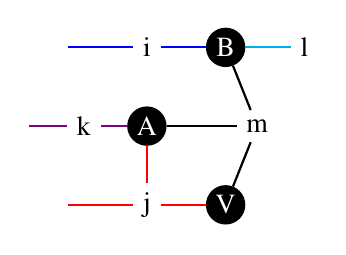
\begin{tikzpicture}[
    dot/.style = {circle, fill, minimum size=#1,
                inner sep=0pt, outer sep=0pt},
    dot/.default = 6pt  % size of the circle diameter 
                    ]  
    \def\dx{0};
    \def\r{0.5cm}
    \def\sr{0.15cm}
    \def\ax{0}
    \def\ay{0}
    \def\bx{1}
    \def\by{1}
    \def\cx{1}
    \def\cy{-1}
    \node[color=white,fill=black,dot=\r] at (\ax+\dx,\ax) (a) {A};
    \node[color=white,fill=black,dot=\r] at (\bx+\dx,\by) (b) {B};
    \node[color=white,fill=black,dot=\r] at (\cx+\dx,\cy) (v) {V};
    \node[color=transparent,draw=transparent,dot=0] at (\ax-1,\by) (o1) {};
    \node[color=transparent,draw=transparent,dot=0] at (\ax-1.5,\ay) (o2) {};
    \node[color=transparent,draw=transparent,dot=0] at (\ax-1,\cy) (o3) {};
    \node at (\ax-0.8,\ay) (k) {k};
    \node at (\bx+0.4,\ay) (m) {m};
    \node at (\ax,\cy) (j) {j};
    \node at (\bx+1,\by) (l) {l};
    \node at (\bx-1,\by) (i) {i};
    \draw[color=blue,thick] (i) -- (b);
    \draw[color=blue,thick] (i) -- (o1);
    \draw[color=cyan,thick] (l) -- (b);
    \draw[color=violet,thick] (k) -- (a);
    \draw[color=violet,thick] (k) -- (o2);
    \draw[color=black,thick] (b) -- (m);
    \draw[color=black,thick] (m) -- (a);
    \draw[color=black,thick] (m) -- (v);
    \draw[color=red,thick] (a) -- (j);
    \draw[color=red,thick] (v) -- (j);
    \draw[color=red,thick] (o3) -- (j);
\end{tikzpicture}}
\end{example}

\section{Generic programming tensor contractions}\label{sec:generic}
In previous works relating tensor networks and combinatoric problems~\cite{Kourtis2019, Biamonte2017},
the elements in the tensor networks are limited to standard number types such as floating point numbers and integers.
Owning to the development of modern compiling technology, we no longer need to limit our imagination to standard number types.
One of the key concepts that push the technology forward is called generic programming:

\begin{definition}[Generic programming ~\cite{Stepanov2014}]
   Generic programming is an approach to programming that focuses on designing algorithms and data structures so that they work in the most general setting without loss of efficiency.
\end{definition}

This definition of generic programming contains two major aspects: a single program works in the most general setting and efficiency.
To understand the first aspect on generality, suppose we want to write a function that raises an element to a power, $f(x, n) := x^n$.
One can easily write a function for standard number types that computes the power of $x$ in $O \left( \log(n) \right)$ steps using the multiply and square trick.
Generic programming does not require $x$ to be a standard number type,
instead it treats $x$ as an element with an associative multiplication operation $\odot$ and a multiplicative identity $\mymathbb{1}$.
In such a way, when the program takes a matrix as an input, it computes the matrix power without extra efforts.
The second aspect is about performance. For dynamically typed languages such as Python,
one can easily write very general codes, but the efficiency is not guaranteed; for example, the speed of computing the matrix multiplication between two numpy arrays with python objects as elements is much slower than statically typed languages such as C++ and Julia~\cite{Bezanson2012}.
C++ uses templates for generic programming while Julia takes advantage of just-in-time compilation and multiple dispatch.
When these languages ``see'' a new input type, the compiler can recompile the generic program for the new type.
A myriad of optimizations can be done during the compilation, such as inlining immutable elements with fixed sizes in an array to decrease the cache miss rate when accessing data.
In Julia, these inlined arrays can even be compiled to GPU devices for faster computation~\cite{Besard2018}.

This motivates us to think about what is the most general element type allowed in a tensor network contraction program.
We find that as long as the algebra of tensor elements forms a commutative semiring, the tensor network contraction result will be valid and be independent of the contraction order.
A commutative semiring is a ring with its multiplication operation being commutative and without an additive inverse.
To define a commutative semiring with the addition operation $\oplus$ and the multiplication operation $\odot$ on a set $R$, the following relations must hold for any arbitrary three elements $a, b, c \in R$.
\begin{align*}
(a \oplus b) \oplus c = a \oplus (b \oplus c) & \hspace{5em}\text{$\triangleright$ commutative monoid $\oplus$ with identity $\mymathbb{0}$}\\
a \oplus \mymathbb{0} = \mymathbb{0} \oplus a = a &\\
a \oplus b = b \oplus a &\\
&\\
(a \odot b) \odot c = a \odot (b \odot c)  &   \hspace{5em}\text{$\triangleright$ commutative monoid $\odot$ with identity $\mymathbb{1}$}\\
a \odot  \mymathbb{1} =  \mymathbb{1} \odot a = a &\\
a \odot b = b \odot a &\\
&\\
a \odot (b\oplus c) = a\odot b \oplus a\odot c  &  \hspace{5em}\text{$\triangleright$ left and right distributive}\\
(a\oplus b) \odot c = a\odot c \oplus b\odot c &\\
&\\
a \odot \mymathbb{0} = \mymathbb{0} \odot a = \mymathbb{0}
\end{align*}
We require the algebra being multiplicative commutative because the contraction order optimizer will change the multiplication order of elements, while we wish this contraction order does not change the contraction results.
In the following sections, we show how to compute a number of properties of independent sets by designing tensor element types as specific commutative semirings without changing the tensor network contraction program~\cite{Stepanov2014}.
The Table~\ref{tbl:generictypes} summarizes those properties that can be computed by various tensor element types.

\begin{table}[t!]\centering
\begin{minipage}{\columnwidth}
\ra{1.3}
        \begin{tabularx}{\textwidth}{sb}\toprule
            \hline
   \textbf{element type}     & \textbf{property to compute} \\
   {$\mathbbm{R}$}     & {the number of independent sets} \\
   {Polynomial} (\Eq{eq:polynomial})     & {independence polynomial} \\
   {Tropical (\Eq{eq:tropical})}    & {MIS size} \\
   {Polynomial truncated to highest order (\Eq{eq:countingtropical})}     & {MIS size and the number of MISs} \\
   {Polynomial truncated to 2nd highest order} (\Eq{eq:max2poly})     & {the number of MISs and independent sets of size $\alpha(G)-1$} \\
   {Set} (\Eq{eq:set})     & {enumeration of independent sets} \\
   {Bit string} (\Eq{eq:singleconfig})     & {one independent set} \\
   {Polynomial truncated to highest order combined with Bit string}     & {MIS size and one MIS} \\
   {Polynomial truncated to highest order combined with Set} (\Eq{eq:countingtropicalset})    & {MIS size and all MISs} \\
            \bottomrule
        \end{tabularx}
    \caption{Tensor element types and the independent set properties that can be computed using them.}\label{tbl:generictypes}
\end{minipage}
\end{table}

\section{Tensor network representation of independent sets} \label{sec:tnmap}
Let $G=(V,E)$ be a weighted graph with each vertex $i\in V$ being associated with a weight $w_i$.
We map a vertex $i\in V$ to a label $s_i \in \{0, 1\}$ of dimension $2$ in a tensor network, where we use $0$ ($1$) to denote a vertex is absent (present) in the set.
For each label $s_i$, we defined a parametrized rank-one vertex tensor $W(x_i, w_i)$ as
\begin{equation}
    W(x_i, w_i) = \left(\begin{matrix}
        1 \\
        x_i^{w_i}
    \end{matrix}\right).
\end{equation}
We use subscripts to index tensor elements, e.g.\ $W(x_i, w_i)_0=1$ is the first element associated with $s_i=0$ and $W(x_i, w_i)_1=x_i^{w_i}$ is the second element associated with $s_i=1$.
Similarly, on each edge $(u, v)$, we define a matrix $B$ indexed by $s_u$ and $s_v$ as
\begin{equation}
    \qquad \quad 
       B = \left(\begin{matrix}
        1  & 1\\
        1 & 0
    \end{matrix}\right). \label{eq:edgetensor}
\end{equation}
The corresponding tensor network contraction gives
\begin{equation}\label{eq:idp}
    P(G, \{x_1, x_{2}, \ldots,x_{|V|}\}) = \sum\limits_{s_1, s_2, \ldots, s_{|V|} = 0}^{1} \prod\limits_{i=1}^{|V|} W(x_i, w_i)_{s_i} \prod\limits_{(i,j) \in E(G)} B_{s_i s_j},
\end{equation}
where the summation runs over all vertex configurations $\{s_1, s_{2}, \ldots,s_{|V|}\}$ and accumulates the product of tensor elements to the output $P$ (see Example \ref{eg:tensorcontraction} for a concrete example).
The edge tensor element $B_{s_{i}=1, s_{j}=1} = 0$ encodes the independent set constraint, meaning vertex $i$ and $j$ cannot be both in the independent set if they are connected by an edge $(i,j)$.

To evaluate \Eq{eq:idp}, directly summing up the $2^{|V|}$ product terms is computationally inefficient.
The standard approach to evaluate a tensor network is to contract two tensors at a time with a certain order utilizing the associativity and commutativity of tensor contraction.
A fully optimized contraction order can reduce the time to $O(2^{\text{tw}(G)})$~\cite{Markov2008}, while requiring a space at the same order of magnitude to store intermediate contraction results.
The pairwise tensor contraction also makes it possible to utilize basic linear algebra subprograms (BLAS) functions to speed up the computation for certain tensor element types.

\begin{example}\label{eg:tensorcontraction}
Mapping a graph (left) to a tensor network (right) that encodes the independence polynomial.
In the generalized tensor network's graphical representation, a vertex is mapped to a hyperedge.
We attach a vertex tensor on each hyperedge and an edge tensor between two hyperedges if vertices of the two hyperedges are connected in the original graph.
    
    \centerline{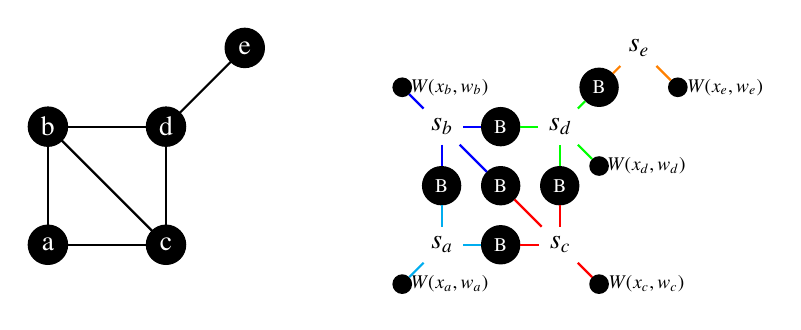
\begin{tikzpicture}[
    dot/.style = {circle, fill, minimum size=#1,
                inner sep=0pt, outer sep=0pt},
    dot/.default = 6pt  % size of the circle diameter 
                    ]  
        \def\dx{0};
        \def\r{0.25cm}
        \filldraw[fill=black] (\dx,0) circle [radius=\r];
        \filldraw[fill=black] (\dx,1.5) circle [radius=\r];
        \filldraw[fill=black] (1.5+\dx,0) circle [radius=\r];
        \filldraw[fill=black] (1.5+\dx,1.5) circle [radius=\r];
        \filldraw[fill=black] (2.5+\dx,2.5) circle [radius=\r];
        \draw [black,thick] (\dx,0) -- (\dx,1.5);
        \draw [black,thick] (\dx,0) -- (1.5+\dx,0);
        \draw [black,thick] (\dx,1.5) -- (1.5+\dx,1.5);
        \draw [black,thick] (1.5+\dx,0) -- (1.5+\dx,1.5);
        \draw [black,thick] (1.5+\dx,0) -- (\dx,1.5);
        \draw [black,thick] (2.5+\dx,2.5) -- (1.5+\dx,1.5);
        \node[color=white] at (\dx,0) {a};
        \node[color=white] at (\dx,1.5) {b};
        \node[color=white] at (1.5+\dx,0) {c};
        \node[color=white] at (1.5+\dx,1.5) {d};
        \node[color=white] at (2.5+\dx,2.5) {e};
        \def\dx{5};
        \def\r{0.25cm}
        \foreach \x/\y/\e in {0.75/0/ac, 0/0.75/ab, 1.5/0.75/cd, 0.75/1.5/bd, 0.75/0.75/bc, 2/2/de}
            \node[color=white,fill=black,dot=2*\r] at (\x+\dx,\y) (\e) {\scriptsize B};
        \foreach \x/\y/\v in {0/0/a, 0/1.5/b, 1.5/0/c, 1.5/1.5/d, 2.5/2.5/e}
            \node[color=black] at (\x+\dx,\y) (\v) {$s_\v$};
        \foreach \x/\y/\v in {-0.5/-0.5/a, -0.5/2.0/b, 2.0/-0.5/c, 2.0/1.0/d, 3.0/2.0/e}
            \node[color=white,fill=black,dot=\r] at (\x+\dx,\y) (\v\v) {};
        \foreach \x/\y/\v in {-0.5/-0.5/a, -0.5/2.0/b, 2.0/-0.5/c, 2.0/1.0/d, 3.0/2.0/e}
            \node[color=black] at (\x+\dx+0.6,\y) {\scriptsize $W(x_\v, w_\v)$};
        \draw [cyan,thick] (a) -- (aa);
        \draw [cyan,thick] (a) -- (ab);
        \draw [cyan,thick] (a) -- (ac);
        \draw [blue,thick] (b) -- (bb);
        \draw [blue,thick] (b) -- (ab);
        \draw [blue,thick] (b) -- (bc);
        \draw [blue,thick] (b) -- (bd);
        \draw [red,thick] (c) -- (cc);
        \draw [red,thick] (c) -- (ac);
        \draw [red,thick] (c) -- (bc);
        \draw [red,thick] (c) -- (cd);
        \draw [green,thick] (d) -- (dd);
        \draw [green,thick] (d) -- (bd);
        \draw [green,thick] (d) -- (de);
        \draw [green,thick] (d) -- (cd);
        \draw [orange,thick] (e) -- (ee);
        \draw [orange,thick] (e) -- (de);
    \end{tikzpicture}}
    
    The contraction of this tensor network can be done in a pairwise order utilizing the associativity, additive commutativity, and multiplicative commutativity of tensor elements:
    \small{
    \begin{align*}
        &\sum_{s_a,s_b,s_c,s_d,s_e} W(x_a, w_a)_{s_a} W(x_b, w_b)_{s_b} W(x_c, w_c)_{s_c} W(x_d, w_d)_{s_d} W(x_e, w_e)_{s_e} B_{s_a s_b} B_{s_b s_d} B_{s_c s_d} B_{s_a s_c} B_{s_b s_c} B_{s_d s_e}\\
        =&\sum_{s_b,s_c}\left(\sum_{s_d}\left(\left(\left(\left(\sum_{s_e}B_{s_d s_e}W(x_e,w_e)_{s_e}\right) W(x_d,w_d)_{s_d}\right) \left(B_{s_bs_d} W(x_b, w_b)_{s_b}\right)\right) \left(B_{s_cs_d} W(x_c, w_c)_{s_c}\right)\right)\right.\\
        &\phantom{XXX}\left.\left(B_{s_bs_c}\left(\sum_{s_a}B_{s_as_b}\left(B_{s_as_c}W(x_a,w_a)_{s_a}\right)\right)\right)\right)\\
        =&1 + x_a^{w_a} + x_b^{w_b} + x_c^{w_c} + x_d^{w_d} + x_e^{w_e} + x_a^{w_a}x_d^{w_d} + x_a^{w_a}x_e^{w_e} + x_c^{w_c}x_e^{w_e} + x_b^{w_b}x_e^{w_e}\\
        =&1+5x+4x^2 \qquad \quad (x_{i} = x, w_{i}=1).
    \end{align*}}
\end{example}

\section{Independence polynomial}\label{sec:indpoly}
In the special case of $x_i = x$ and $w_i = 1$, the contraction result directly corresponds to the independence polynomial.
The independence polynomial is an important graph polynomial that contains the counting information of independent sets. It is defined as
\begin{equation}\label{eq:idpdef}
I(G, x) = \sum_{k=0}^{\alpha(G)} a_k x^k,
\end{equation}
where $a_k$ is the number of independent sets of size $k$ in graph $G=(V,E)$. The total number of independent sets is thus equal to $I(G, 1)$.
Its connection to \Eq{eq:idp} can be understood as follows: the product over vertex tensor elements produces a factor $x^k$, where $k=\sum_i s_i$ counts the set size,
and the product over edge tensor elements gives a factor $1$ for a configuration being in an independent set and $0$ otherwise. The summation counts the number of independent sets of size $k$. 
One can feed the standard computer numbers types into this tensor network and evaluate the independence polynomial by contracting it numerically.
However, we are more interested in finding the coefficients of this polynomial, because this quantity tells us the counting of independent sets at each size.
To achieve this, let us first elevate the tensor elements $0$s and $1$s in tensors $W(x, 1)$ and $B$ from integers and floating point numbers to the additive identity,
$\mymathbb{0}$, and multiplicative identity, $\mymathbb{1}$, of a commutative semiring as discussed in Sec.~\ref{sec:generic}.
Let us create a polynomial type and represent a polynomial $a_0 + a_1 x + \ldots + a_k x^k$ as a coefficient vector $a = (a_0, a_1, \ldots, a_k) \in \mathbb{R}^k$, so, e.g., $x$ is represented as $(0, 1)$.
We define the algebra between the polynomials $a$ of order $k_a$ and $b$ of order $k_b$ as
\begin{equation}
    \eqname{PN}
    \begin{split}
    a \oplus b &= (a_0 + b_0, a_1 + b_1, \ldots, a_{\max(k_a, k_b)} + b_{\max(k_a, k_b)}),\\
    a \odot b &= (a_0 + b_0, a_1b_0 + a_0b_1, a_{2}b_{0} + a_{1}b_{1} + a_{0}b_{2},  \ldots, a_{k_a} b_{k_b}),\\
    \mymathbb{0} &= (),  \\
    \mymathbb{1} &= (1).\label{eq:polynomial}
    \end{split}
\end{equation}
Here, the multiplication operation can be evaluated efficiently using the convolution theorem~\cite{Schonhage1971}.
These operations are standard addition and multiplication operations of polynomials, and the polynomial type forms a commutative ring. The tensors $W$ and $B$ can thus be written as 
\begin{equation}
    W^{\rm PN} = \left(\begin{matrix}
        \mymathbb{1} \\
        (0,1)
    \end{matrix}\right),   
    \qquad \qquad
        B^{\rm PN} = \left(\begin{matrix}
        \mymathbb{1}  & \mymathbb{1} \\
        \mymathbb{1} & \mymathbb{0}
    \end{matrix}\right).
\end{equation}
By contracting the tensor network with the polynomial type, we have the exact representation of the independence polynomial.
In practise, using the polynomial type suffers a space overhead proportional to $\alpha(G)$ because each polynomial requires a vector of such size to store the coefficients. 
Here, we propose to find the independence polynomial by fitting $\alpha(G)+1$ random pairs of $x_{i}$ and $y_{i} = I(G,x_{i})$. One can then compute the independence polynomial coefficients $a_{i}$ by solving the linear equation: 
\begin{equation}
\left(\begin{matrix}
1 & x_0 & x_0^2 & \ldots & x_0^{\alpha(G)} \\
1 & x_1 & x_1^2 & \ldots & x_1^{\alpha(G)} \\
\vdots & \vdots & \vdots &\ddots & \vdots \\
1 & x_{\alpha(G)} & x_{\alpha(G)}^2 & \ldots & x_{\alpha(G)}^{\alpha(G)}
\end{matrix}\right)
\left(\begin{matrix}
a_0 \\ a_1 \\ \vdots \\ a_{\alpha(G)}
\end{matrix}\right)
= \left(\begin{matrix}
y_0 \\ y_1 \\ \vdots \\ y_{\alpha(G)}
\end{matrix}\right).\label{eq:lineareq}
\end{equation}
With this approach, we do not incur the linear overhead in space. However, because the independence polynomial coefficients can have a huge order-of-magnitude range, if we use floating point numbers in the computation, the round-off errors can be significant for the counting of large-size independent sets.
In addition, the number could easily overflow if we use fixed-width integer types.
The big integer type is also not a good option because big integers with varying width can be very slow and is incompatible with GPU devices. These problems can be solved by introducing a finite-field algebra $\text{GF}(p)$:
\begin{equation}
\eqname{GF$(p)$}
\begin{split}
    x ~\oplus~ y &= x+y\pmod p,\\
    x ~\odot~ y &= xy\pmod p,\\
    \mymathbb{0} &= 0,\\
    \mymathbb{1} &= 1.
\end{split}\label{eq:finitefield}
\end{equation}
With a finite-field algebra, we have the following observations:
\begin{enumerate}
    \item One can use Gaussian elimination~\cite{Golub2013} to solve the linear equation \Eq{eq:lineareq} since it is a generic algorithm that works for any elements with field algebra. The multiplicative inverse of a finite-field algebra can be computed with the extended Euclidean algorithm.
    \item Given the remainders of a larger unknown integer $x$ over a set of co-prime integers $\{p_1, p_2, \ldots, p_n\}$,
    $x \pmod {p_1 \times p_2 \times \ldots \times p_n}$ can be computed using the Chinese remainder theorem. With this, one can infer big integers from small integers.
\end{enumerate}
With these observations, we develop Algorithm~\ref{alg:finitefield} to compute the independence polynomial exactly without introducing space overheads.
The algorithm iterates over a sequence of large prime numbers until convergence.
In each iteration, we choose a large prime number $p$, and contract the tensor networks to evaluate the polynomial for each variable $\chi = (x_{0}, x_{1}, \ldots, x_{\alpha(G)})$ on ${\rm GF}(p)$ and denote the outputs as $(y_0, y_1, \ldots, y_{\alpha(G)}) \pmod p$.
Then we solve \Eq{eq:lineareq} using Gaussian elimination on ${\rm GF}(p)$ to find the coefficient modulo $p$, $A_p \equiv (a_0, a_1, \ldots, a_{\alpha(G)})\pmod p$.
As the last step of each iteration, we apply the Chinese remainder theorem to update $A \pmod P $ to $ A \pmod {P\times p}$, where $P$ is a product of all prime numbers chosen in previous iterations.
If this number does not change compared with the previous iteration, it indicates the convergence of the result and the program terminates.
All computations are done with integers of fixed width $W$ except the last step of applying the Chinese remainder theorem, where we use arbitrary precision integers to represent the counting.
In \App{app:fft}, we provide another method to solve the linear equation using discrete Fourier transformation.

\LinesNumberedHidden
\begin{algorithm}[!ht]
    \small
    \SetAlgoNoLine
    %\LinesNumbered
    Let $P = 1$, $W$ be the integer width, vector $\chi = (0,1,2, \ldots, \alpha(G))$, matrix $X_{ij} = (\chi_i)^j$, where $i,j = 0, 1, \ldots, \alpha(G)$\;

    \While{true}{
        compute the largest prime $p$ that $\gcd(p, P) = 1$ and $p < 2^W$\;

        \For{$i=0\ldots\alpha(G)$}{
            $y_i \pmod p$ = ${\rm contract\_tensor\_network}(\chi_i\pmod p)$ \tcp*[l]{on $\text{GF}(p)$}
        }

        $A_p = (a_0, a_1, \ldots, a_{\alpha(G)}) \pmod p = {\rm gaussian\_elimination}(X, (y_0, y_1, \ldots, y_{\alpha(G)}) \pmod p) $\;

        $A_{P\times p} = {\rm chinese\_remainder}(A_P, A_p)$\;

        \If{$A_P = A_{P \times p}$}{
            \Return $A_P$ \tcp*[l]{converged}
        }
        $P = P \times p$\;
    }\caption{Computing the independence polynomial exactly without integer overflow}\label{alg:finitefield} 
\end{algorithm}

\section{Maximum independent sets and its counting}\label{sec:counting}
\subsection{Tropical algebra for finding the MIS size and counting MISs}
In the previous section, we focused on computing the independence polynomial for a graph $G$ of a given MIS size $\alpha(G)$, but we did not show how to compute this number.
The method we use to compute this quantity is based on the following observations. Let $x=\infty$, the independence polynomial becomes
\begin{equation}
I(G, \infty) = a_{\alpha(G)} \infty^{\alpha(G)},
\end{equation}
where the lower-order terms vanish. We can thus replace the polynomial type $a = (a_0, a_1, \ldots, a_k)$ with a new type with two fields: the largest exponent $k$ and its coefficient $a_k$.
From this, we can define a new algebra as
\begin{equation}
    \eqname{P1}
\begin{split}
    a_x\infty^x \oplus a_y\infty^y &= \begin{cases}
        (a_x + a_y)\infty^{\max(x,y)}, & x = y\\
        a_y\infty^{\max(x,y)}, & x < y\\
        a_x\infty^{\max(x,y)}, & x > y
    \end{cases}, \\
    a_x\infty^x \odot a_y\infty^y &= a_x a_y\infty^{x+y}\\
    \mymathbb{0} &= 0\infty^{-\infty}\\
    \mymathbb{1} &= 1\infty^{0}.
\end{split}%& \text{\rlap{(P1)}}
\label{eq:countingtropical}
\end{equation}
To implement this algebra programmatically, we create a data type with two fields $(x, a_x)$ to store the MIS size and its counting,
and define the above operations and constants correspondingly.
If one is only interested in finding the MIS size, one can drop the counting field.
The algebra of the exponents becomes the max-plus tropical algebra~\cite{Maclagan2015, Moore2011}:
\begin{equation}\eqname{T}
    \begin{split}
        x \oplus y &= \max(x,y)\\
        x \odot y &= x + y\\
        \mymathbb{0} &= -\infty\\
        \mymathbb{1} &= 0.
    \end{split}\label{eq:tropical}
\end{equation}
This algebra is the same as the one used in Liu et al.~\cite{Liu2021} to calculate and count spin glass ground states.
For independent set calculations here, the vertex tensor and edge tensor becomes:
\begin{equation}
    W^{\rm T} = \left(\begin{matrix}
        \mymathbb{1} \\
        \infty
    \end{matrix}\right),   
    \qquad \qquad
        B^{\rm T} = \left(\begin{matrix}
        \mymathbb{1}  & \mymathbb{1} \\
        \mymathbb{1} & \mymathbb{0}
    \end{matrix}\right).
\end{equation}

\subsection{Truncated polynomial algebra for counting independent sets of large size}
Instead of counting just the MISs, one may be interested in counting the independent sets of large sizes close to the MIS size.
For example, if one is interested in counting only $a_{\alpha(G)}$ and $a_{\alpha(G)-1}$, we can define a truncated polynomial algebra by keeping only the largest two coefficients in the polynomial in \Eq{eq:polynomial} as:
\begin{equation}
    \eqname{P2}
    \begin{split}
    a \oplus b &= (a_{\max(k_a, k_b)-1} + b_{\max(k_a, k_b)-1}, a_{\max(k_a, k_b)} + b_{\max(k_a, k_b)}),\\
    a \odot b &= (a_{k_a-1} b_{k_b}+a_{k_a} b_{k_b-1}, a_{k_a} b_{k_b}),\\
    \mymathbb{0} &= (), \\
    \mymathbb{1} &= (1).\label{eq:max2poly}
    \end{split}
\end{equation}
In the program, we thus need a data structure that contains three fields, the largest order $k$, and the coefficients for the two largest orders $a_k$ and $a_{k-1}$.
This approach can clearly be extended to calculate more independence polynomial coefficients and is more efficient than calculating the entire independence polynomial.
As will be shown below, this algebra can also be extended to enumerate those large-size independent sets.

\section{Enumerating and sampling independent sets}\label{sec:enumeration}
\subsection{Set algebra for configuration enumeration}
The enumeration problems of independent sets are also interesting and has been studied extensively in the literature~\cite{Bron1973, Eppstein2010, Johnson1988}, including,
for example, the enumeration of all independent sets, the enumeration of all maximal independent sets, or the enumeration of all MISs.
To enumerate all independent sets, we designed an algebra defined on sets of bitstrings:
\begin{equation}
\eqname{SN}
\begin{split}
    s \oplus t &= s \cup t\\
    s \odot t &= \{\sigma \lor^\circ \tau \, | \, \sigma \in s, \tau \in t\}\\
    \mymathbb{0} &= \{\}\\
    \mymathbb{1} &= \{0^{\otimes |V|}\}.
\end{split}\label{eq:set}
\end{equation}
where $s$ and $t$ are each a set of $|V|$-bit strings and $\lor^\circ$ is the bitwise OR operation over two bit strings.
\begin{example}\label{eg:setalgebra}
    For elements being bit strings of length $5$, we have the following set algebra
\begin{equation*}
\begin{split}
    &\{00001\} \oplus \{01110, 01000\} = \{01110, 01000\} \oplus \{00001\} = \{00001,01110, 01000\}\\
    &\{00001\} \oplus \{\} = \{00001\}\\
&\\
    &\{00001\} \odot \{01110, 01000\} = \{01110, 01000\} \odot \{00001\} = \{01111, 01001\}\\
    &\{00001\} \odot \{\} = \{\}\\
    &\{00001\} \odot \{00000\} = \{00001\}.
\end{split}
\end{equation*}
\end{example}

To enumerate all independent sets, 
we initialize variable $x_{i}$ in the vertex tensor to $x_i = \{\boldsymbol{e}_{i}\}$, where $\boldsymbol{e}_i$ is a basis bit string of size $|V|$ that has only one non-zero value at location $i$.
The vertex and edge tensors are thus
\begin{equation}
    W^{\rm SN}(\{\boldsymbol{e}_{i}\}) = \left(\begin{matrix}
        \mymathbb{1} \\
        \{\boldsymbol{e}_{i}\}
    \end{matrix}\right),   
    \qquad \qquad
        B^{\rm SN} = \left(\begin{matrix}
        \mymathbb{1}  & \mymathbb{1} \\
        \mymathbb{1} & \mymathbb{0}
    \end{matrix}\right).
\end{equation}

This set algebra can serve as the coefficients in \Eq{eq:polynomial} to enumerate independent sets of all different sizes, \Eq{eq:countingtropical} to enumerate all MISs,
or \Eq{eq:max2poly} to enumerate all independent sets of size $\alpha(G)$ and $\alpha(G)-1$.
As long as the coefficients in a truncated polynomial forms a commutative semiring, the polynomial itself is still a commutative semiring.
For example, to enumerate only the MISs, with the tropical algebra, we can define $s_{k}\infty^k$,
where the coefficients follow the algebra in \Eq{eq:set} and the orders (exponents) follow the max-plus tropical algebra.
The combined operations become: 
\begin{equation}
\eqname{P1+SN}
\begin{split}
    s_x\infty^x \oplus s_y\infty^y &= \begin{cases}
        (s_x \cup s_y)\infty^{\max(x,y)}, & x = y\\
        s_y\infty^{\max(x,y)}, & x < y\\
        s_x\infty^{\max(x,y)}, & x > y
    \end{cases},\\
    s_x\infty^x \odot s_y\infty^y &= \{\sigma \lor^\circ \tau | \sigma \in s_x, \tau \in s_y\}\infty^{x+y},\\
    \mymathbb{0} &= \{\}\infty^{-\infty},\\
    \mymathbb{1} &= \{0^{\otimes |V|}\}\infty^{0}. \label{eq:countingtropicalset}
\end{split}
\end{equation}
Clearly, the vertex tensor and edge tensor become
\begin{equation}
    W^{\rm P1+SN}(\{\boldsymbol{e}_{i}\infty^1\}) = \left(\begin{matrix}
        \mymathbb{1} \\
        \{\boldsymbol{e}_{i}\}\infty^1
    \end{matrix}\right),   
    \qquad \qquad
        B^{\rm P1+SN} = \left(\begin{matrix}
        \mymathbb{1}  & \mymathbb{1} \\
        \mymathbb{1} & \mymathbb{0}
    \end{matrix}\right).
\end{equation}
The contraction of the corresponding tensor network yields an enumeration of all MIS configurations.

If one is interested in obtaining only a single MIS configuration, one can just keep a single configuration in the intermediate computations to save the computational effort.
Here is a new algebra defined on the bit strings, replacing the sets of bit strings in \Eq{eq:set}, 

\begin{equation}
\eqname{S1}
\begin{split}
    \sigma \oplus \tau &= {\rm select}(\sigma, \tau), \\
    \sigma \odot \tau &= (\sigma\lor^\circ \tau),\\
    \mymathbb{0} &= 1^{\otimes |V|}, \\
    \mymathbb{1} &= 0^{\otimes |V|},
\end{split}\label{eq:singleconfig}
\end{equation}
where the \texttt{select} function picks one of $\sigma$ and $\tau$ by some criteria to make the algebra commutative and associative, e.g. by picking the one with a smaller integer value.

\subsection{Bounding the MIS enumeration space}
\begin{figure}
    \centering
    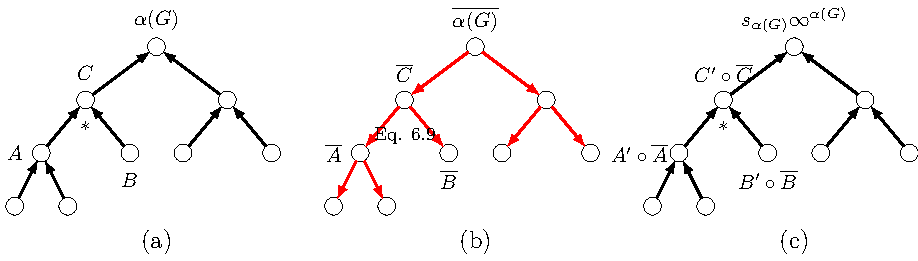
\includegraphics[width=0.9\textwidth, trim={0cm 0cm 0cm 0cm}, clip]{figures/masktree.pdf}
    \caption{Bounded enumeration of maximum independent sets. In these graphs, a circle is a tensor, an arrow specifies execution direction of a function and $\circ$ is the Hadamard (element-wise) multiplication. $\overline A$ means the boolean mask of $A$. (a) is the forward pass with algebra \Eq{eq:tropical} for computing $\alpha(G)$.
     (b) is the backward pass for computing boolean gradients as masks.
     (c) is the masked forward pass with algebra \Eq{eq:countingtropicalset} for enumerating configurations.}
     \label{fig:bounding}
\end{figure}

When we use the algebra in \Eq{eq:countingtropicalset} to enumerate all MIS configurations, we find that the program stores significantly more intermediate configurations than necessary and thus incur significant overheads in space.
To speed up the computation and reduce space overhead, we bound the searching space using the information from the computation of the MIS size $\alpha(G)$.
As shown in \Fig{fig:bounding}, (a) we first compute the value of $\alpha(G)$ with tropical algebra and cache all intermediate tensors.
(b) Then, we compute a boolean mask for each cached tensor, where we use a boolean true to represent a tensor element having a contribution to the MIS (i.e.\ with a non-zero gradient) and boolean false otherwise.
(c) Finally, we perform masked tensor network contraction (i.e.\ discarding the unnecessary intermediate configurations) using the element type with the algebra in \Eq{eq:countingtropicalset} to obtain all MIS configurations.
Note that these masks in fact correspond to tensor elements with non-zero gradients with respect to the MIS size; we compute these masks by back propagating the gradients.
To derive the back-propagation rule for tropical tensor contraction,
we first reduce the problem to finding the back-propagation rule of a tropical matrix multiplication $C = A B$.
Since $ C_{ik} = \bigoplus_{j} \ A_{ij} \odot B_{jk} = \max_{j} \ A_{ij} \odot B_{jk}$ with tropical algebra, we have the following inequality
\begin{equation}
    A_{ij} \odot B_{jk} \leq C_{ik}.
\end{equation}
Here $\leq$ on tropical numbers are the same as the real-number algebra.
The equality holds for some $j'$, which means $A_{ij'}$ and $B_{j'k}$ have contributions to $C_{ik}$.
Intuitively, one can use this relation to identify elements with nonzero gradients in $A$ and $B$,
but if doing this directly, one loses the advantage of using BLAS libraries~\cite{TropicalGEMM} for high performance.
Since $A_{ij} \odot B_{jk} = A_{ij} + B_{jk}$, one can move $B_{jk}$ to the right hand side of the inequality: 
\begin{equation}
    A_{ij} \leq C_{ik} \odot B_{jk}^{\circ -1}
\end{equation}
where ${}^{\circ -1}$ is the element-wise multiplicative inverse on tropical algebra (which is the additive inverse on real numbers).
The inequality still holds if we take the minimum over $k$: 
\begin{equation}
    A_{ij} \leq \min_{k}(C_{ik} \odot B_{jk}^{\circ -1}) = \left(\max_{k} \left(C_{ik}^{\circ -1} \odot B_{jk} \right) \right)^{\circ -1} = \left(\bigoplus_{k} \left(C_{ik}^{\circ -1} \odot B_{jk} \right) \right)^{\circ -1} = \left( C^{\circ-1} B^{\mathsf{T}} \right)^{\circ -1}_{ij}.
\end{equation}
On the right hand side, we transform the operation into a tropical matrix multiplication so that we can utilize the fast tropical BLAS routines~\cite{TropicalGEMM}.
Again, the equality holds if and only if the element $A_{ij}$ has a contribution to $C$ (i.e.\ having a non-zero gradient).
Let the gradient mask for $C$ be $\overline C$; the back-propagation rule for gradient masks reads
\begin{equation}\label{eq:adrule}
\overline{A}_{ij} = \delta \left(A_{ij}, \left( \left( C^{\circ-1} \circ \overline C \right) B^{\mathsf{T}} \right)_{ij}^{\circ -1} \right),
\end{equation}
where $\delta$ is the Dirac delta function that returns one if two arguments have the same value and zero otherwise, $\circ$ is the element-wise product, boolean false is treated as the tropical number $\mymathbb{0}$, and boolean true is treated as the tropical number $\mymathbb{1}$.
This rule defined on matrix multiplication can be easily generalized to tensor contraction by replacing the matrix multiplication between $C^{\circ-1} \circ \overline C$ and $B^{\mathsf{T}}$ by a tensor contraction.
With the above method, one can significantly reduce the space needed to store the intermediate configurations by setting the tensor elements masked false to zero during contraction.

\subsection{Extremely large MIS enumeration space}
In many times, the number of configurations is too large to fit into any type of storage.
Then instead of using the set algebra, we can use a binary sum-product tree as a compact representation of the results.
We use a quadruple $(type, data, left, right)$ to represent a node in the tree, where $type$ is one of
$\{\texttt{LEAF}, \texttt{ZERO}, \texttt{SUM}, \texttt{PROD}\}$, $data$ is a bit string as the content is a \texttt{LEAF} node,
$left$ and $right$ are left and right operands of \texttt{SUM} and \texttt{PROD} nodes.

\begin{equation}
\eqname{EXPR}
\begin{split}
    s \oplus t &= (\texttt{SUM}, /, s, t)\\
    s \odot t &= (\texttt{PROD}, /, s, t)\\
    \mymathbb{0} &= (\texttt{ZERO}, /, /, /)\\
    \mymathbb{1} &= (\texttt{LEAF}, 0^{\otimes |V|}, /, /).
\end{split}\label{eq:expr}
\end{equation}

This algebra is a commutative semiring because we define the equivalence of two sum-product trees by comparing their expanded (using \Eq{eq:set}) forms, rather than their storages.
Although one is probably unable to enumerate the configurations represented by this tree due to the extremely large configuration space size,
but he can directly sample configurations from this tree.
This is because once we have this sum-product representation of the configuration space,
one can compute the number of configurations in each branch rigorously and efficiently.
One can generate a random number and descent this expression tree by a probability proportional to the size of left and right branches.

\section{Weighted graphs}\label{sec:weighted}
In the previous discussion, we have limited ourselves to unweighted graphs.
For integer weighted graphs, all results still holds,
while for general weighted graphs, the independence polynomial is not computable anymore.
For general weighted graphs, we are more interested to know the total weights of maximum $k$ independent set sizes and their configurations.
Hence we define the extended tropical numbers as the following

\begin{equation}
\eqname{Tk}
\begin{split}
    s \oplus t &= \texttt{largest}(s \cup t, k)\\
    s \odot t &= \texttt{largest}(\{a+b| a \in s, b\in t\}, k)\\
    \mymathbb{0} &= -\infty^{\otimes k}\\
    \mymathbb{1} &= -\infty^{\otimes k-1} \otimes 0
\end{split}\label{eq:ext-tropical}
\end{equation}
where $\texttt{largest}(s, k)$ means truncating the set by only keeping $k$ largest values in the set $s$.
Similarly, we can attach a bit string sampler algebra \Eq{eq:singleconfig} to it for finding the configuration for each size.
Note here, the $\odot$ of configuration sampler is not used so that the resulting configurations are complete.

\section{Performance benchmarks}\label{sec:benchmark}
We run a single thread benchmark on CPU Intel(R) Xeon(R) CPU E5-2686 v4 @ 2.30GHz,
and its CUDA version on a GPU Tesla V100-SXM2 16G.
The results are summarized in Figure~\ref{fig:benchmark}.
The graphs that we use in benchmarks are random three regular graphs,
 a typical type of sparse graphs that has a small treewidth that asymptotically smaller than $|V|/6$~\cite{Fomin2006}.

\begin{figure} 
    \centering
    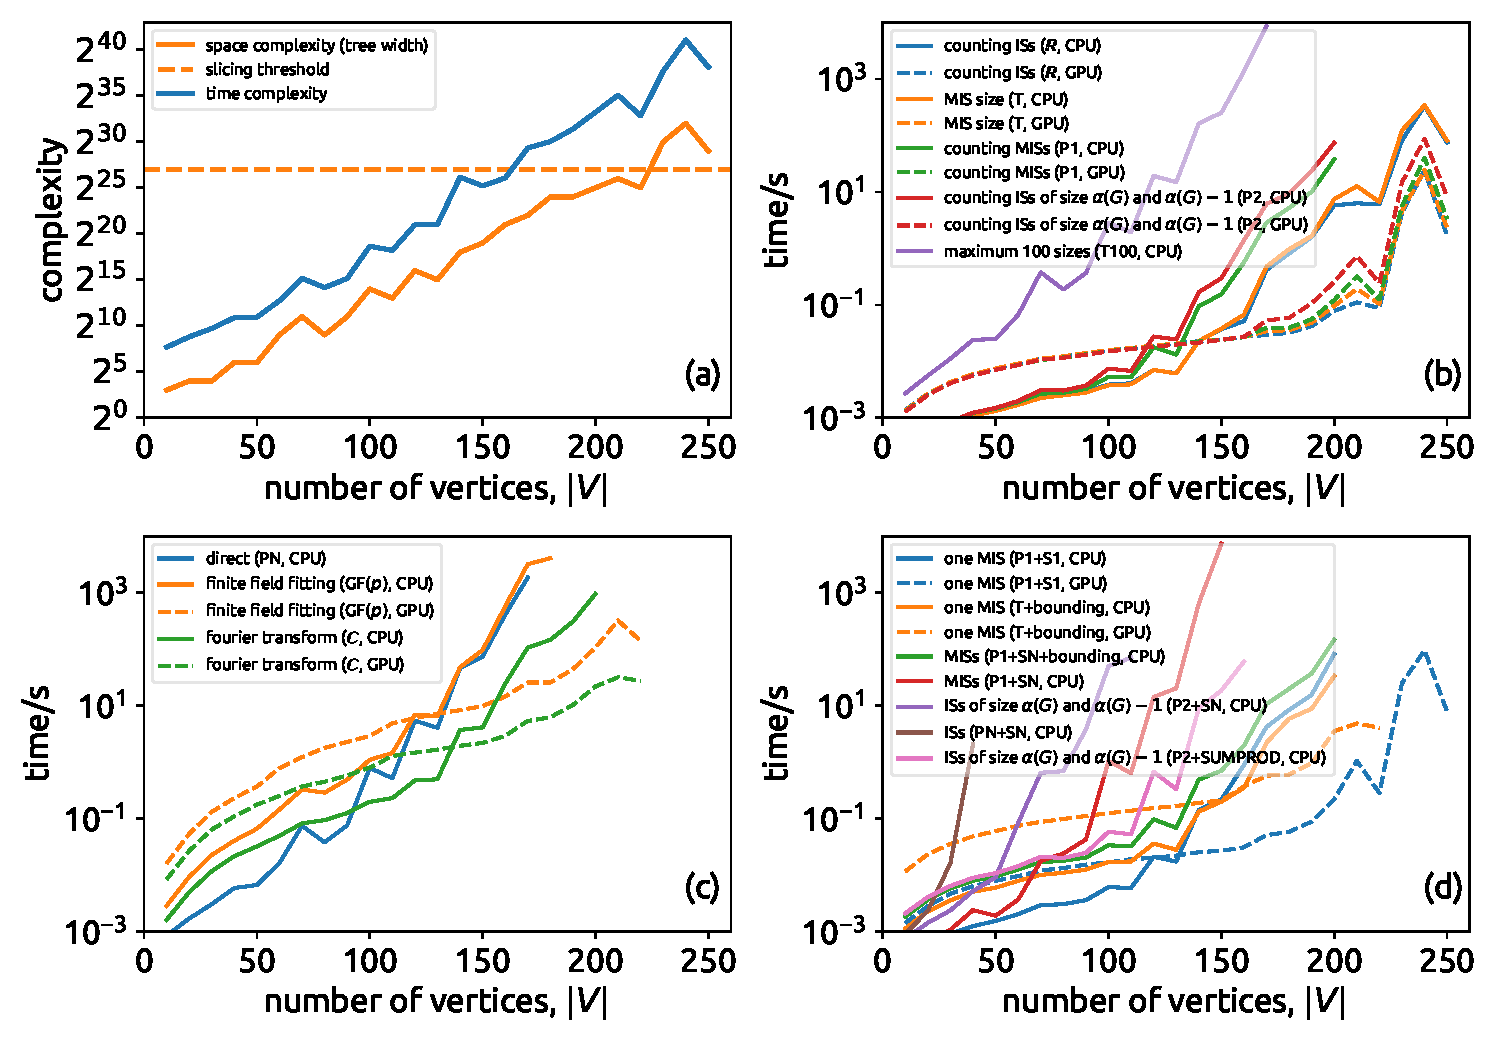
\includegraphics[width=\textwidth, trim={0cm 0cm 0cm 0cm}, clip]{figures/fig1.pdf}
    \caption{Benchmark results for computing different properties of independent sets of a random three regular graph with different tensor element types.
    The time in these plots only includes tensor network contraction, without taking into account the contraction order finding and just-in-time compilation time.
    Legends are properties, algebra and devices that we used in the computation; one can find the corresponding computed property in \Tbl{tbl:generictypes}.
    (a) time and space complexity versus the number of vertices for the benchmarked graphs.
    (b) The computing time for calculating the MIS size and for counting of the number of all independent sets (ISs), the number of MISs, and the number of independent sets having size $\alpha(G)$ and $\alpha(G)-1$.
    (c) The computing time for calculating the independence polynomials with different approaches.
    (d) The computing time for configuration enumeration, including the enumeration of all independent set configurations, a single MIS configuration, all MIS configurations, all independent set configurations having size $\alpha(G)$ and $\alpha(G)-1$,  with or without bounding the enumeration space.
    }
    \label{fig:benchmark}
\end{figure}

Figure~\ref{fig:benchmark}(a) shows the time and space complexity of tensor network contraction for different graph sizes, where the space complexity is the same as the treewidth of the problem graph.
The contraction order is obtained using the local search algorithm in Ref.~\cite{Kalachev2021}.
In practice, slicing technique is used for graphs with treewidth greater than 27 to fit the computation into a 16GB memory.
One can see that all the computing times in figure~\ref{fig:benchmark}(b), (c) and (d) have a strong correlation with the treewidth.
Among these benchmarks, computational tasks with data types \texttt{T (CPU)},
\texttt{$\mathbbm{R}$ (CPU)}, \texttt{$\mathbbm{R}$ (GPU)}, \texttt{$\mathbbm{C}$ (CPU)}, \texttt{$\mathbbm{C}$ (GPU)} and \texttt{T+bounding (CPU)} can utilize fast BLAS functions to evaluate tensor contractions, hence 
are much faster comparing to non-BLAS element types in the same category.
GPU computes much faster than CPU in all cases when the problem scale is large enough such that the actual computing time is comparable or larger than the launching overhead of CUDA kernels.
Most algebras can be computed on a GPU, except those requiring dynamic sized structures, i.e.\ \texttt{PN} and \texttt{SN}.
In figure~\ref{fig:benchmark}(c), one can see the Fourier transformation based method is the fastest in computing the independence polynomial,
but it may suffer from round-off errors. The finite field (GF$(p)$) approach is the only method that does not have round-off errors and can be run on a GPU.
In figure~\ref{fig:benchmark}(d), one can see the technique to bound the enumeration space improves the performance for more than one order of magnitude in enumerating the MISs.
Bounding can also reduce the memory usage significantly, without which the largest computable graph size is only $\sim150$ on a device with 32GB main memory.

\section{Example case studies} \label{sec:examples}
In this section, we give a few examples where the different properties of independence sets are used.

\subsection{Number of independent sets and entropy constant for some hardcore lattice gases}\label{sec:entropy}
We compute the counting of all independent sets for graphs shown in Figure~\ref{fig:lattices}, where vertices are all placed on square lattices with lattice dimensions $L \times L$.
The types of graphs include: the square grid graphs (Figure~\ref{fig:lattices}(a)); the square grid graphs with a filling factor $p=0.8$, which means $\lfloor pL^{2} \rceil$ square grids are occupied with vertices  (Figure~\ref{fig:lattices}(b));
the King's graphs  (Figure~\ref{fig:lattices}(c)); the King's graphs with a filling factor $p = 0.8$  (Figure~\ref{fig:lattices}(d)).
The number of independent sets for square grid graphs of size $L \times L$ form a well-known integer sequence (\href{https://oeis.org/A006506}{OEIS A006506}), which is thought as a two-dimensional generalization of the Fibonacci numbers.
We computed the integer sequence for $L=38$ and $L=39$, which, to the best of our knowledge, is not known before.
In the computation, we used the finite-field algebra for contracting arbitrarily high precision integer tensor networks. 

A useful number that can be computed using the number of independent sets is the entropy constant for the hardcore lattice gases on these graphs. For the square grid graphs, it is called the \textit{hard square entropy constant} (\href{https://oeis.org/A085850}{OEIS A085850}), which is defined as $\lim_{L\rightarrow \infty} F(L,L)^{1/L^2}$, where $F(L,L)$ is the number of independent sets of a given lattice dimensions $L \times L$. This quantity arises in statistical mechanics of hard-square lattice gases~\cite{Baxter1980, Pearce1988} and is used to understand phase transitions for these systems. This entropy constant is not known to have an exact representation, but it is accurately known in many digits. Similarly, we can define entropy constants for other lattice gases. In \Fig{fig:hardsquare}, we look at how $F(L,L)^{1/\lfloor pL^2\rceil}$ scales as a function of the grid size $L$ for all types of graphs shown in Figure~\ref{fig:lattices}. Our results match the known results for the non-disordered square grid and King's graphs. For disordered square grid and King's graphs with a filling factor $p=0.8$, we randomly sample 1000 graph instances. To our knowledge, the entropy constants for these disordered graphs have not been studied before. Interestingly, the variations due to different random instances are negligible for this entropy quantity. 

\begin{figure}[t] 
    \centering
    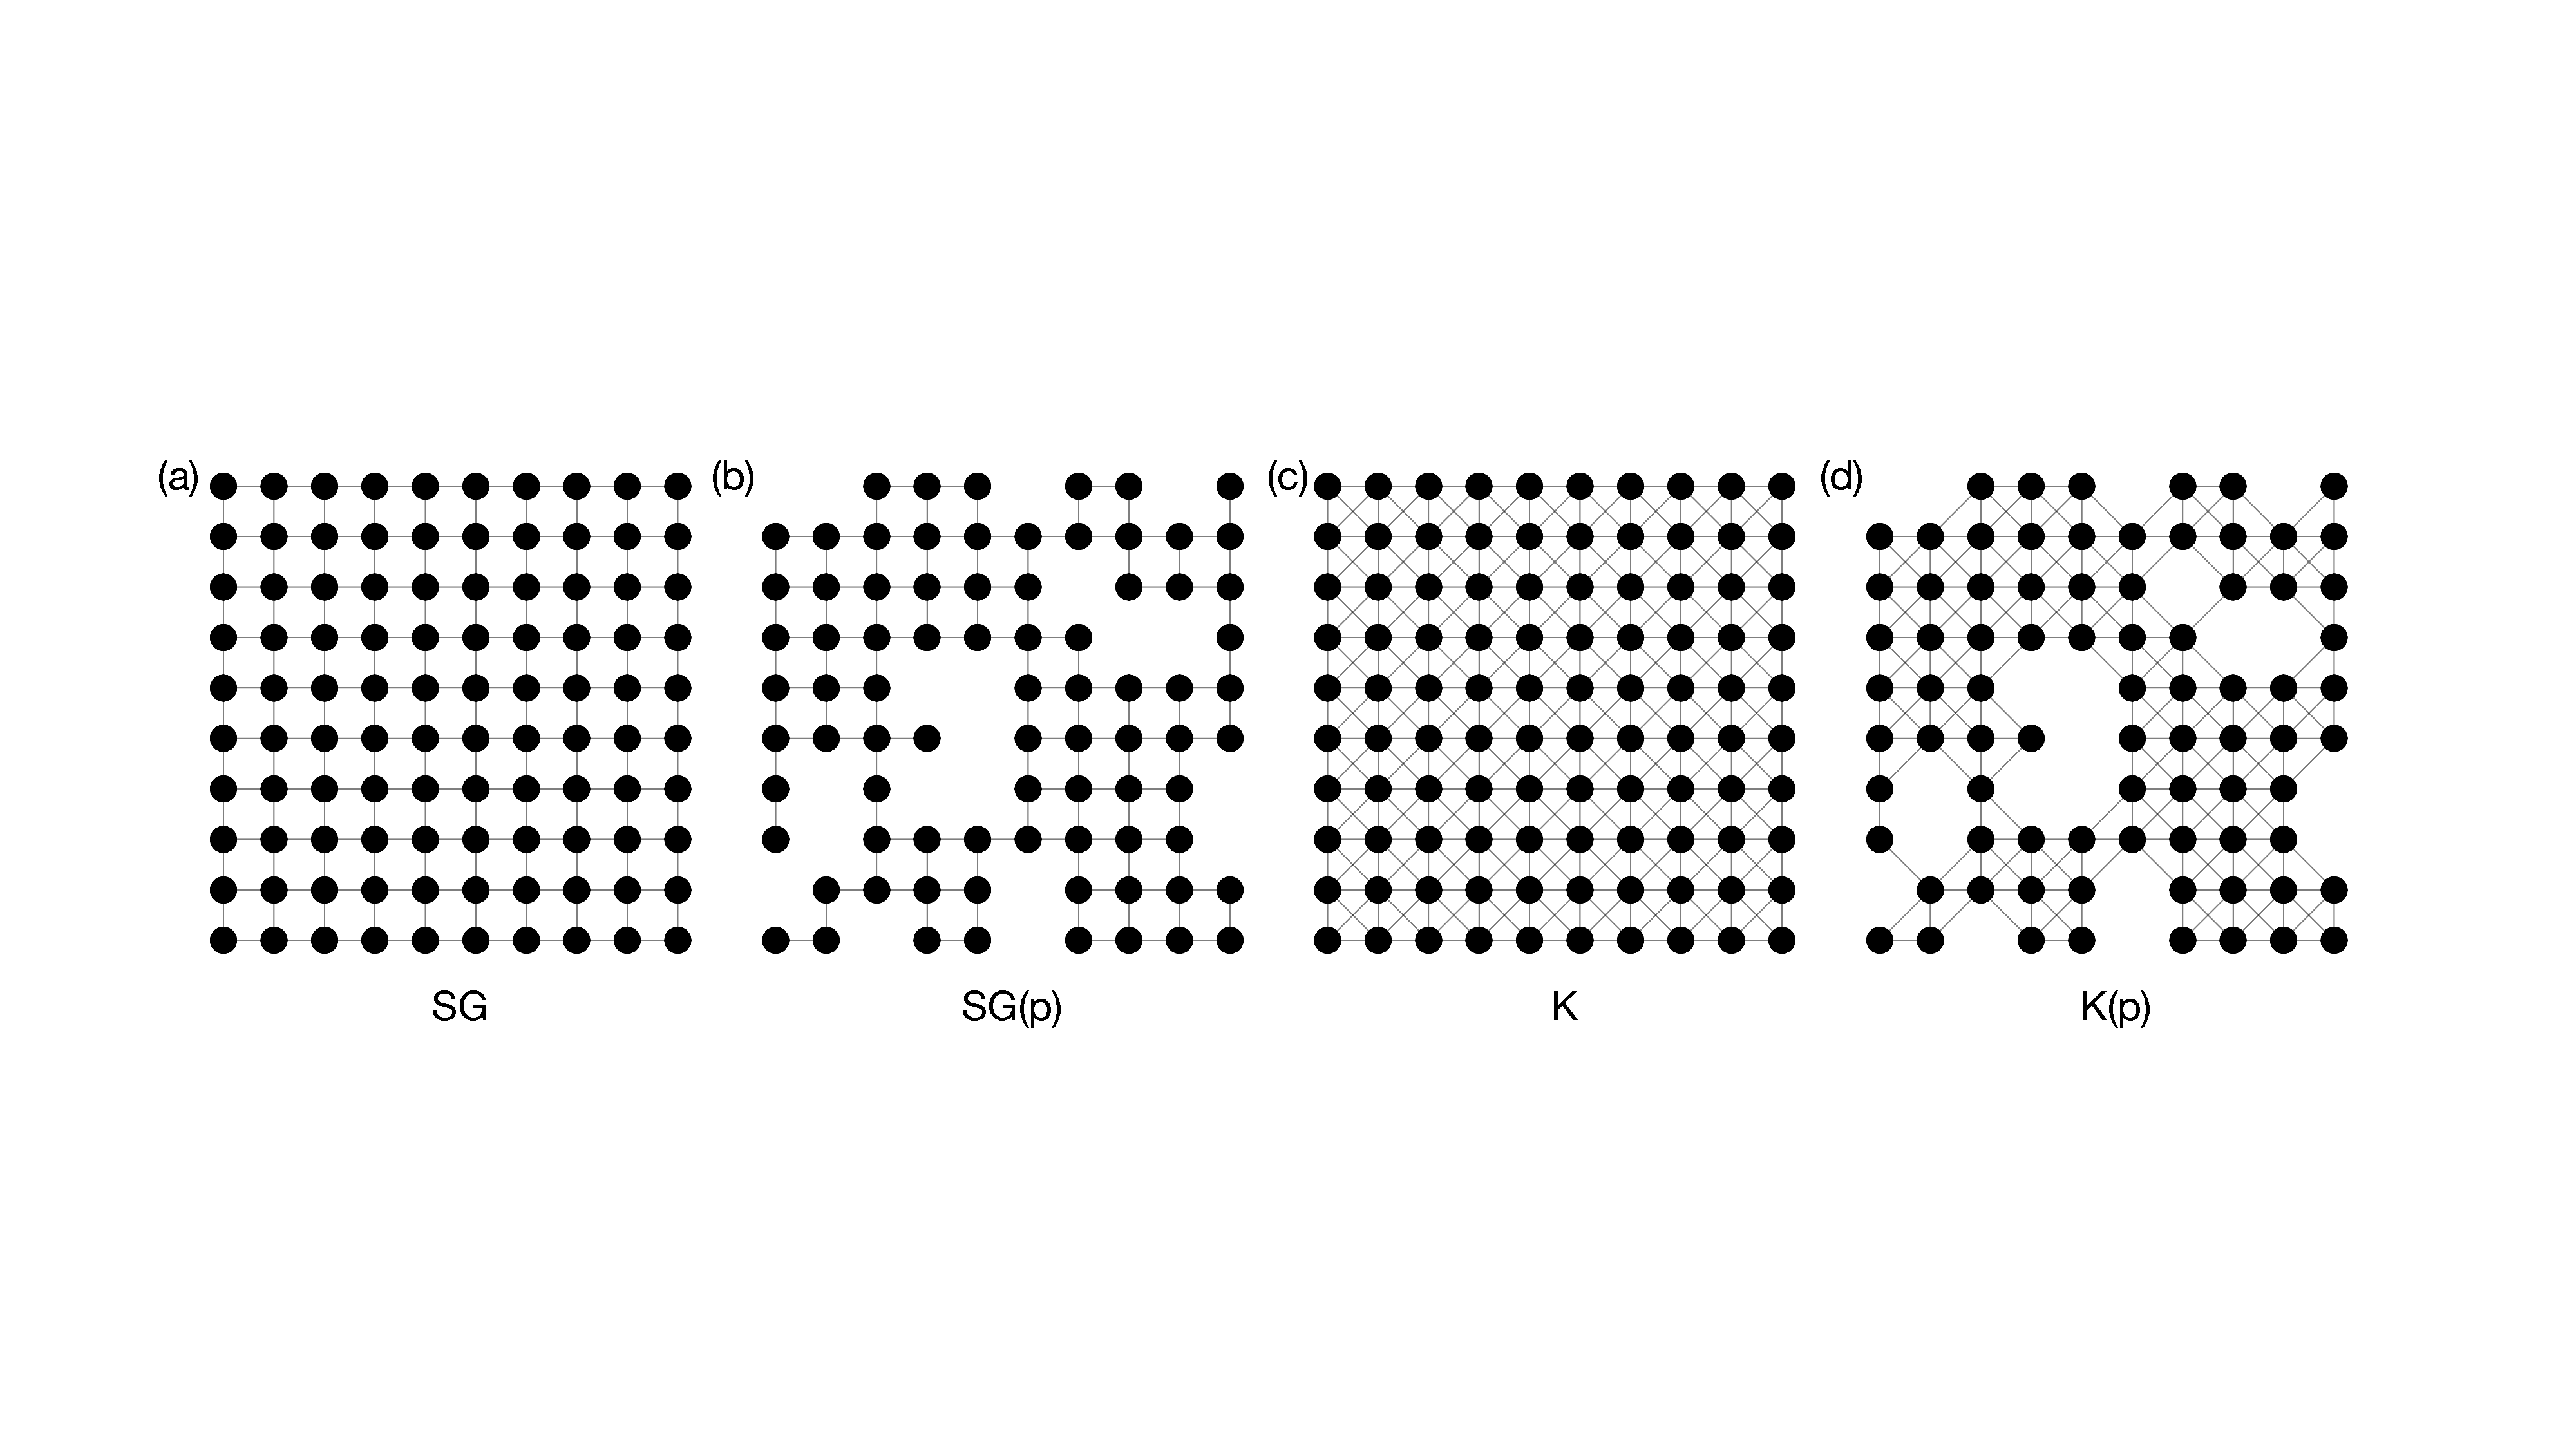
\includegraphics[width=\textwidth, trim={0cm 0cm 0cm 0cm}, clip]{lattices.pdf}
    \caption{The types of graphs used in the case study in section \ref{sec:entropy}.
    The lattice dimensions are $L\times L$. (a) Square grid graphs. (b) Square grid graphs with a filling factor $p=0.8$.
    (c) King's graphs. (d) King's graphs with a filling factor $p=0.8$.}
    \label{fig:lattices}
\end{figure}

\begin{figure}[t] 
    \centering
    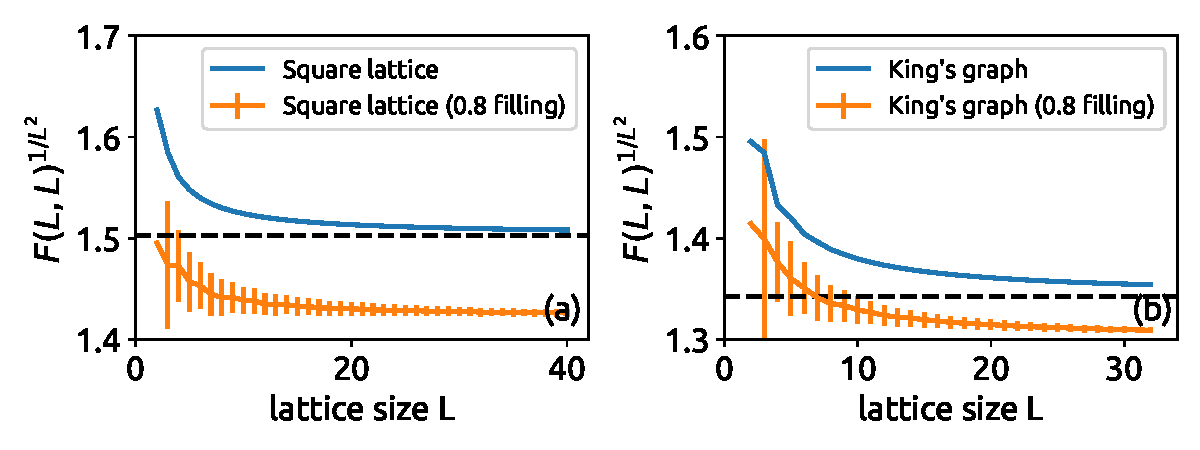
\includegraphics[width=\textwidth, trim={0cm 0cm 0cm 0cm}, clip]{figures/fig5.pdf}
    \caption{Mean entropy for lattice gases on graphs defined in \Fig{fig:lattices}.
    We sampled $1000$ instances for $p=0.8$ lattices and the error bar is too small to be visible.
    The horizontal black dashed lines are for $\lim_{L\rightarrow \infty} F(L,L)^{1/L^2}$ for the corresponding non-disordered square grid and King's graphs.
    }
    \label{fig:hardsquare}
\end{figure}

\subsection{The overlap gap property}
With the tool to enumerate configurations, one can try to understand the structure of the independent set configuration space, such as the optimization landscape for finding the MISs and the geometry of the solution space. One of the known barriers for finding the MIS is the so-called overlap gap property~\cite{Gamarnik2013, Gamarnik2019}. Intuitively, if the overlap gap property is present, it means every two large independent sets either have a significant intersection or very small intersection; it implies that large independent sets are clustered together. This clustering property has been used to prove the limitations of local algorithms in finding the MISs~\cite{Gamarnik2013, Gamarnik2019}. Here, we use the computed configurations of large independent sets to investigate the presence or absence of the overlap gap property for some given graphs. In particular, in \Fig{fig:hamming}, we enumerated all ISs of size $\geq\alpha(G)-1$ for two random three regular graph instances of size 100 and show the pairwise Hamming distance statistics for the enumerated configurations. In \Fig{fig:hamming}(a), we observed the multiple peak structure for the pairwise Hamming distance for one of the graphs. This indicates the presence of the overlap gap property and disconnected clusters exist in the configuration space for large independent sets. We expect our numerical tool can be used to understand this phenomenon better and to further investigate the graph properties and the geometry of the configuration spaces for a variety of graph instances.
\begin{figure} 
    \centering
    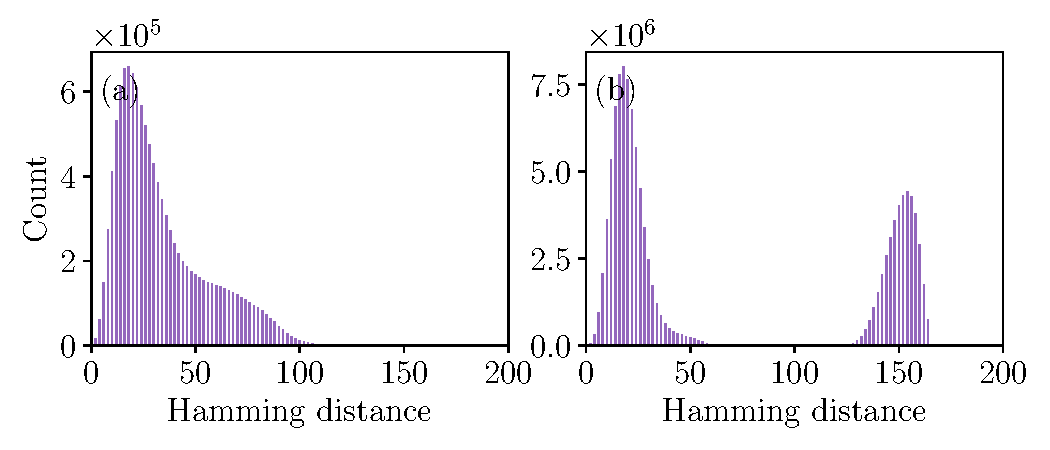
\includegraphics[width=\textwidth, trim={0cm 0cm 0cm 0cm}, clip]{figures/fig3.pdf}
    \caption{The distribution of pairwise Hamming distances between every two independent sets of size $\geq\alpha(G)-1$ for two random three regular graph instances of size $100$.}
    \label{fig:hamming}
\end{figure}

\section{Discussion and conclusion}
In this paper, we introduce a method to use generic programming tensor networks to compute a number of different independent set properties, including the size of the MISs and the number and enumeration of independent sets of a given size. For each property, we design an algebra of a commutative semiring with a particular element type and map the computation of the property to the contraction of a tensor network with such an element type. The data types introduced in the main text can be represented in the following diagram, where we use overlap to represent two algebras that can be combined to create a new algebra.

\begin{figure}[th]
   \centering
\centerline{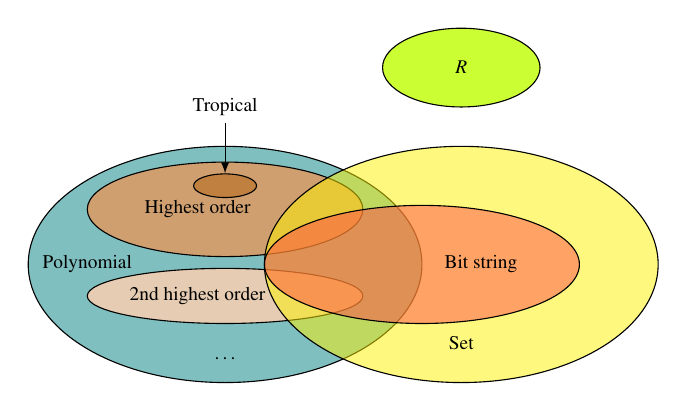
\begin{tikzpicture}[]
    \scriptsize
    \node[draw,fill=lime!80,fill opacity=1, text opacity=1.0,ellipse,minimum width=2cm, minimum height=1cm,inner sep=0pt] at (0, 2.5) (R) {$\mathbbm{R}$};
    \def\dx{-3};
    \node[draw,fill=teal!50,fill opacity=1, text opacity=1.0,ellipse,minimum width=5cm, minimum height=3cm,inner sep=0pt] at (\dx, 0) (PN) {\hspace{-3.5cm}Polynomial};
    \node[draw,fill=brown!75,fill opacity=1, text opacity=1.0,ellipse,minimum width=3.5cm, minimum height=1.2cm,inner sep=0pt] at (\dx, 0.7) (P1) {\hspace{-0.7cm}Highest order};
    \node[draw,fill=brown!40,fill opacity=1, text opacity=1.0,ellipse,minimum width=3.5cm, minimum height=0.7cm,inner sep=0pt] at (\dx, -0.4) (P2) {\hspace{-0.7cm}2nd highest order};
    \node[draw,fill=brown,fill opacity=1, text opacity=1.0,ellipse,minimum width=0.8cm, minimum height=0.3cm,inner sep=0pt] at (\dx, 1.0) (T) {};
    \node at (\dx, -1.2) {$\ldots$};
    \node[above of=2] at (T) (textT) {Tropical};
    \draw[black,-latex] (textT) -- (T);

    % set and set sampler
    \node[draw,fill=yellow,fill opacity=0.5, text opacity=1.0,ellipse,minimum width=5cm, minimum height=3cm,inner sep=0pt] at (0, 0) (SN) {};
    \node[below of=1] at (SN) {Set};
    \node[draw,fill=red!70,fill opacity=0.5, text opacity=1.0,ellipse,minimum width=4cm, minimum height=1.5cm,inner sep=0pt] at (-0.5, 0) (S1) {\hspace{1.5cm}Bit string};
\end{tikzpicture}}

    \caption{The the tensor network element types used in this work.
    The overlap between two algebra indicates that a new algebra can be created by combining those two types of algebra.}
     \label{fig:venn-diagram}
\end{figure}

Other than the case with real numbers, we have polynomials and truncated polynomials as algebra types.
We combine them with the set algebra and the bitstring algebra for set enumeration and sampling. 
These algebras are of generic use: they can be utilized to compute properties of maximal independent sets and a variety of other combinatorial problems such as the matching problem, the k-coloring problem, the max-cut problem, and the set packing problem, as detailed in \App{app:otherproblems}. 
Moreover, since the independence polynomial is closely related to the matching polynomial~\cite{Levit2005}, the clique polynomial~\cite{Hoede1994}, and the vertex cover polynomial~\cite{Akbari2013},
our algorithm to compute the independence polynomial can also be used to compute these graph polynomials.
By adapting to the style of generic programming, we can implement all the algorithms without much effort.
We show some of the Julia language implementations in Appendix~\ref{sec:technical}.
A complete implementation can be found in our Github repository~\cite{GraphTensorNetworks}. 
We expect our tool can be used to understand and study many interesting applications of independent sets and beyond. We also hope this approach of generic tensor networks can inspire future works on tensor network computations.

\section*{Acknowledgments}
We would like to thank Pan Zhang for sharing his python code for optimizing contraction orders of a tensor network.
We acknowledge Sepehr Ebadi, Maddie Cain, and Leo Zhou for coming up with many interesting questions about independent sets and their questions strongly motivated the development of this project.
We thank Chris Elord for helping us to write the fastest matrix multiplication library for tropical numbers, TropicalGEMM.jl. % he is a man of speed!
We would also like to thank a number of open-source software developers, including Roger Luo, Time Besard, and Katharine Hyatt, for solving some implementation issues voluntarily.
\blue{funding information}

\bibliographystyle{siamplain}
\bibliography{refs}

\appendix

\section{Technical guide}\label{sec:technical}
This project depends on multiple open source packages in the Julia ecosystem.
We list the Julia packages that play important roles in our code base as follows:

\begin{description}
	\item[\href{https://github.com/under-Peter/OMEinsum.jl}{OMEinsum} and \href{https://github.com/Happy-Diode/OMEinsumContractionOrders.jl}{OMEinsumContractionOrders}] are packages providing the support for Einstein's (or tensor network) notation and contraction order optimizations.
    \texttt{OMEinsumContractionOrders} implements state-of-the-art algorithms for finding the optimal contraction order for a tensor network, including the KaHypar+Greedy~\cite{Gray2021, Pan2021} and local transformation based approaches~\cite{Kalachev2021},
	\item[\href{https://github.com/TensorBFS/TropicalNumbers.jl}{TropicalNumbers} and \href{https://github.com/TensorBFS/TropicalGEMM.jl}{TropicalGEMM}] are packages providing tropical number and efficient tropical matrix multiplication,
	\item[\href{https://github.com/JuliaGraphs/Graphs.jl}{Graphs}] is a package providing graph utilities, like random regular graph generator,
	\item[\href{https://github.com/JuliaMath/Polynomials.jl}{Polynomials}] is a package providing polynomial algebra and polynomial fitting,
	\item[\href{https://github.com/scheinerman/Mods.jl}{Mods} and \href{https://github.com/JuliaMath/Primes.jl}{Primes}] are packages providing finite field algebra and prime number generations.
\end{description}

One can install these packages by opening a Julia REPL, type \colorbox{lightgray}{\texttt{]}} to enter the \texttt{pkg>} mode and type, e.g.
\begin{lstlisting}
pkg> add OMEinsum Graphs Mods Primes Polynomials TropicalNumbers OMEinsumContractionOrders
\end{lstlisting}

The reader may find it surprising that the Julia implementation of the algorithms introduced in this work is so short that except the bounding algorithm,
all are contained in this appendix. This is due to the power of generic programming. After installing the required packages, one can open a Julia REPL and copy the following codes into it.

\lstinputlisting[breaklines]{../democode/demo.jl}

For better performance, we recommend checking our GitHub repository for the full featured version:
\href{https://github.com/Happy-Diode/GraphTensorNetworks.jl}{https://github.com/Happy-Diode/GraphTensorNetworks.jl}.
It can be installed in a similar style to other packages.

\section{Additional contraction overhead using the standard tensor network notations}\label{app:tensorbad}
As we have mentioned in the main text,
a standard tensor network notation is equivalent to the generalized tensor network by introducing $\delta$ tensors,
where a $\delta$ tensor of rank $d$ is defined as
\begin{equation}
    \delta_{i_1, i_2,\ldots,i_d} = \begin{cases}
        1, & i_1=i_2=\ldots =i_d,\\
        0, & \text{otherwise}.
    \end{cases}
\end{equation}

Let us consider the following King's graph.

\centerline{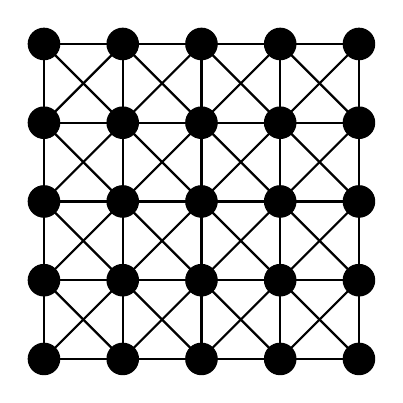
\begin{tikzpicture}
    \def\r{0.2}
    \foreach \x in {1,...,5}
        \foreach \y in {1,...,5}
            \filldraw[fill=black] (\x,\y) circle [radius=\r];
    \foreach \x in {1,...,5}
        \foreach \y in {1,...,4}{
            \draw [black,thick] (\x,\y) -- (\x,\y+1);
            \draw [black,thick] (\y,\x) -- (\y+1,\x);
        }
    \foreach \x in {1,...,4}
        \foreach \y in {1,...,4}{
            \draw [black,thick] (\x,\y) -- (\x+1,\y+1);
            \draw [black,thick] (\y+1,\x) -- (\y,\x+1);
        }
\end{tikzpicture}}

By mapping the independent set problem to a standard tensor network, we have the following graphical representation.

\centerline{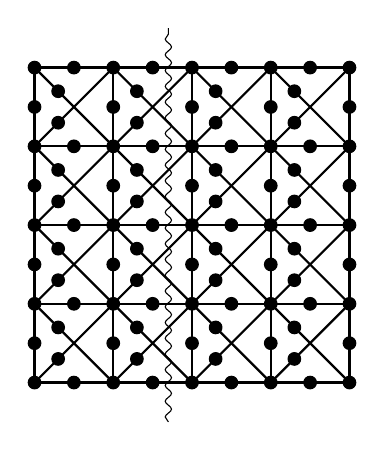
\begin{tikzpicture}
    \def\r{0.08}
    \def\a{0.1}
    \foreach \x in {1,...,5}
        \foreach \y in {1,...,5}
            \filldraw[fill=black] (\x,\y) circle [radius=\r];
    \foreach \x in {1,...,5}
        \foreach \y in {1,...,4}{
            \filldraw[fill=black] (\x,\y+0.5) circle [radius=\r];
            \filldraw[fill=black] (\y+0.5,\x) circle [radius=\r];
            \draw [black,thick] (\x,\y) -- (\x,\y+1);
            \draw [black,thick] (\y,\x) -- (\y+1,\x);
        }
    \foreach \x in {1,...,4}
        \foreach \y in {1,...,4}{
            \filldraw[fill=black] (\x+0.3,\y+0.3) circle [radius=\r];
            \filldraw[fill=black] (\y+0.3,\x+0.7) circle [radius=\r];
            \draw [black,thick] (\x,\y) -- (\x+1,\y+1);
            \draw [black,thick] (\y+1,\x) -- (\y,\x+1);
        }
    \tikzset{decoration={snake,amplitude=.4mm,segment length=2mm,
                    post length=0mm,pre length=0mm}}
    \draw [decorate] (2.7, 0.5) -- (2.7, 5.5);
\end{tikzpicture}}

In this diagram, the circle on each vertex in the original graph is a $\delta$ tensor up to rank $8$.
If we contract this tensor network in a naive column-wise order, the maximum intermediate tensor has rank $\sim3L$, requiring a storage of size $\approx 2^{3L}$.
If we relax the restriction that each label must appears exactly twice, we have the following hypergraph representation of a generalized tensor network.

\centerline{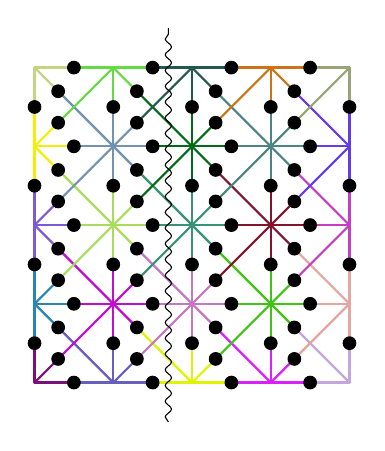
\begin{tikzpicture}
    \def\r{0.08}
    \def\a{0.07}
    \def\L{0.6}
    \def\l{0.1}
    \def\sql{0.24}
    \pgfmathsetseed{2}
    \foreach[evaluate={\cr=0.1+0.5*Mod(\x,2)}] \x in {1,...,5}
        \foreach[evaluate={\cg=0.1+0.3*Mod(\y,2); \cy=0.5-0.5*Mod(\y,2)}] \y in {1,...,5}{
            \edef\R{\pdfuniformdeviate 255}
            \edef\G{\pdfuniformdeviate 255}
            \edef\B{\pdfuniformdeviate 255}
            \xdefinecolor{MyColor}{RGB}{\R,\G,\B}
            \ifnum \x < 5
                \draw [thick, MyColor, opacity=1.0, line cap=round] (\x,\y) -- (\x+0.5,\y);
                \ifnum \y < 5
                \draw [thick, MyColor, opacity=1.0, line cap=round] (\x,\y) -- (\x+0.3,\y+0.3);
                \fi
                \ifnum \y > 1
                \draw [thick, MyColor, opacity=1.0, line cap=round] (\x,\y) -- (\x+0.3,\y-0.3);
                \fi
            \fi
            \ifnum \x > 1
                \draw [thick, MyColor, opacity=1.0, line cap=round] (\x,\y) -- (\x-0.5,\y);
                \ifnum \y < 5
                \draw [thick, MyColor, opacity=1.0, line cap=round] (\x,\y) -- (\x-0.7,\y+0.7);
                \fi
                \ifnum \y > 1
                \draw [thick, MyColor, opacity=1.0, line cap=round] (\x,\y) -- (\x-0.7,\y-0.7);
                \fi
            \fi
            \ifnum \y < 5
                \draw [thick, MyColor, opacity=1.0, line cap=round] (\x,\y) -- (\x,\y+0.5);
            \fi
            \ifnum \y > 1
                \draw [thick, MyColor, opacity=1.0, line cap=round] (\x,\y) -- (\x,\y-0.5);
            \fi
        }
    \foreach \x in {1,...,5}
        \foreach \y in {1,...,5}{
            %\filldraw[fill=black] (\x,\y) circle [radius=0.7*\r];
        }
    \foreach \x in {1,...,5}
        \foreach \y in {1,...,5}{
            \ifnum \y < 5
                \filldraw[fill=black] (\x,\y+0.5) circle [radius=\r];
                \filldraw[fill=black] (\y+0.5,\x) circle [radius=\r];
            \fi
        }
    \foreach \x in {1,...,4}
        \foreach \y in {1,...,4}{
            \filldraw[fill=black] (\x+0.3,\y+0.3) circle [radius=\r];
            \filldraw[fill=black] (\y+0.3,\x+0.7) circle [radius=\r];
        }
    \tikzset{decoration={snake,amplitude=.4mm,segment length=2mm,
                    post length=0mm,pre length=0mm}}
    \draw [decorate] (2.7, 0.5) -- (2.7, 5.5);
\end{tikzpicture}}
Here, we use different colors to distinguish different hyperedges.
A vertex tensor always has rank $1$ and is not shown here since it does not change the contraction complexity.
If we contract this tensor network in the column-wise order, the maximum intermediate tensor rank is $\sim L$, which can be seen by counting the number of colors.

\section{Generalization to other graph problems}\label{app:otherproblems}
\subsection{Maximal independent sets and maximal cliques}\label{sec:maximal}
Finding maximal independent sets of a graph is equivalent to finding the maximal cliques of its complement graph, so in the following we mainly discuss how to find maximal independent sets.
Let us denote the neighborhood of a vertex $v$ as $N(v)$ and denote $N[v] = N(v)\cup \{v\}$.
A maximal independent set $I_m$ is an independent set where there exists no vertex $v \in V$ such that $I_m \cap N[v]  = \emptyset$.
Similar to the independence polynomial, the maximal independence polynomial counts the number of maximal independent sets of various sizes~\cite{Hu2017},
which can be helpful for understanding why the program for solving MIS can be trapped in a local minimum.
Concretely, it is defined as
\begin{equation}
I_{\rm max}(G, x) = \sum_{k=0}^{\alpha(G)} b_k x^k,
\end{equation}
where $b_k$ is the number of maximal independent sets of size $k$ in graph $G=(V, E)$.
Comparing with the independence polynomial in \Eq{eq:idpdef}, we have $b_{k} \leq a_{k}$ and $b_{\alpha(G)} = a_{\alpha(G)}$. $I_{\rm max}(G, 1)$ counts the total number of maximal independent sets~\cite{Gaspers2012, Manne2013}, where, to our knowledge, the fastest algorithm currently has a runtime of $O(1.3642^{|V|})$~\cite{Gaspers2012}.
If we want to find an MIS, $b_{k}$ counts the number of local optimum at size $k < \alpha(G)$, and can, in some cases, provide hints on the difficulty of finding the MIS using local algorithms~\cite{Ebadi2022}.
The uni-modality, log-concavity, and real-rootness properties of the maximal independence polynomial for special classes of graphs have also been studied~\cite{Hu2017}. 

We can modify the tensor network for computing the independence polynomial to include this restriction. Instead of defining the restriction on vertices and edges, it is more natural to define it on $N[v]$:
\begin{equation}\label{eq:maximal}
    T(x_v)_{s_1,s_2,\ldots,s_{|N(v)|},s_v} = \begin{cases}
        s_vx_v & s_1=s_2=\ldots=s_{|N(v)|}=0,\\
        1-s_v& \text{otherwise}.\\
    \end{cases}
\end{equation}
Intuitively, it means if all the neighbourhood vertices are not in $I_{m}$, i.e., $ s_1=s_2=\ldots=s_{|N(v)|}=0$, then $v$ should be in $I_{m}$ and contribute a factor $x_{v}$,
otherwise, if any of the neighbourhood vertices is in $I_{m}$, then $v$ cannot be in $I_{m}$.
As an example, for a vertex of degree 2, the resulting rank-3 tensor is
\begin{equation}
    T(x_v)=\left(\begin{matrix}
    \left(\begin{matrix}
        0 &1 \\
        1 &1
    \end{matrix}\right)\\
    \left(\begin{matrix}
        x_v &0 \\
        0 &0
    \end{matrix}\right)
    \end{matrix}\right).
\end{equation}
 
By contracting this tensor network with generic element types,
we can compute the maximal independent set properties such as the maximal independence polynomial and the enumeration of maximal independent sets.
Let us consider the example in~\Sec{eg:tensorcontraction}: its corresponding tensor network structure for computing the maximal independent polynomial becomes

    \centerline{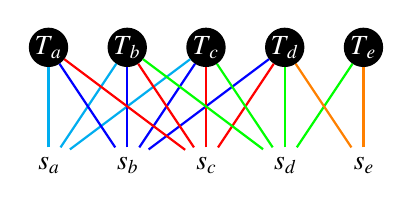
\begin{tikzpicture}[
    dot/.style = {circle, fill, minimum size=#1,
                inner sep=0pt, outer sep=0pt},
    dot/.default = 6pt  % size of the circle diameter 
                    ]  
        \def\dx{0};
        \def\r{0.5cm}
        \def\G{1.0}
        \foreach \x/\y/\v in {0/0/a, 1/0/b, 2/0/c, 3/0/d, 4/0/e}
            \node[color=black] at (\x*\G+\dx,\y) (\v) {$s_\v$};
        \foreach \x/\v/\t in {0/A/$T_a$, 1/B/$T_b$, 2/C/$T_c$, 3/D/$T_d$, 4/E/$T_e$}
            \node[color=white,fill=black,dot=\r] at (\x*\G+\dx,1.5) (\v) {\t};
        \draw [cyan,thick] (a) -- (A);
        \draw [cyan,thick] (a) -- (B);
        \draw [cyan,thick] (a) -- (C);
        \draw [blue,thick] (b) -- (B);
        \draw [blue,thick] (b) -- (A);
        \draw [blue,thick] (b) -- (C);
        \draw [blue,thick] (b) -- (D);
        \draw [red,thick] (c) -- (C);
        \draw [red,thick] (c) -- (A);
        \draw [red,thick] (c) -- (B);
        \draw [red,thick] (c) -- (D);
        \draw [green,thick] (d) -- (D);
        \draw [green,thick] (d) -- (B);
        \draw [green,thick] (d) -- (C);
        \draw [green,thick] (d) -- (E);
        \draw [orange,thick] (e) -- (E);
        \draw [orange,thick] (e) -- (D);
    \end{tikzpicture}}
 
One can see that the average degree of a tensor is increased.
The computational complexity of this new tensor network contraction is often greater than the one for computing the independence polynomial.
However, for most sparse graphs, this tensor network contraction approach is still much faster than enumerating all the maximal cliques on its complement graph using the Bron-Kerbosch algorithm~\cite{Bron1973}, which is the standard algorithm that we are aware of to compute the maximal independence polynomial.
We show the benchmark of computing the maximal independent set properties in \Fig{fig:benchmark-maximal},
including a comparison to the Bron-Kerbosch algorithm from Julia package Graphs~\cite{Graphs}.
The treewidth of this tensor network is significantly larger, so benchmark with only a smaller graph size is feasible.
The time for the tensor network approach and the Bron-Kerbosch approach to enumerate all maximal independent sets are comparable,
while the tensor network does counting much more efficiently.
Due to the memory limit, this Bron-Kerbosch algorithm is only feasible up to a graph size around $70$.

\begin{figure} 
    \centering
    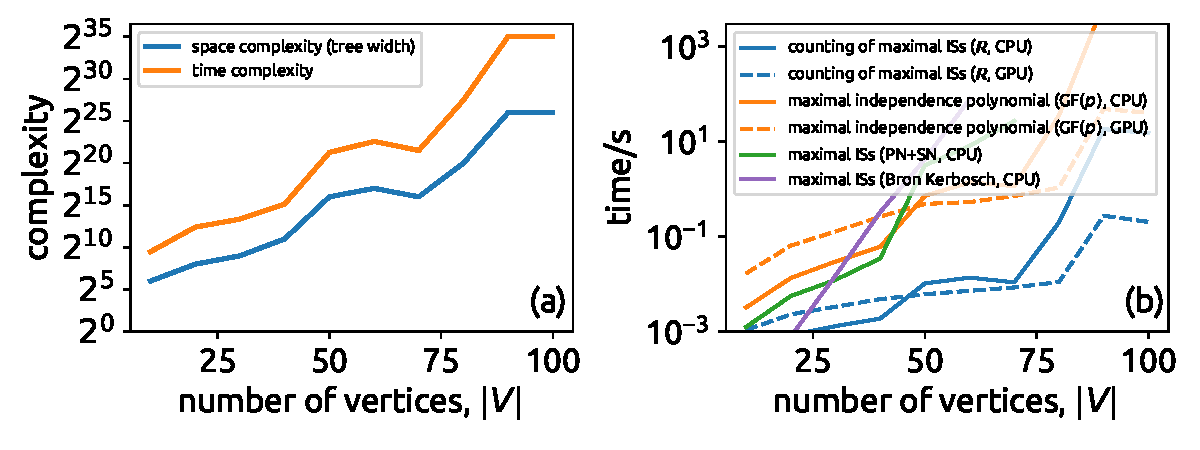
\includegraphics[width=\textwidth, trim={0cm 0cm 0cm 0cm}, clip]{figures/fig2.pdf}
    \caption{Benchmark results for computing different properties of maximal independent sets on a random three regular graph with different tensor element types.
    (a) treewidth versus the number of vertices for the benchmarked graphs. 
    (b) The computing time for calculating the number of independent sets and enumerate all MISs.
    }
    \label{fig:benchmark-maximal}
\end{figure}


\subsection{Matching problem}
A matching polynomial of a graph $G$ is defined as
\begin{equation}
    M(G, x) = \sum\limits_{k=1}^{|V|/2} c_k x^k,
\end{equation}
where $k$ is the size of a matching, and coefficients $c_k$ are the corresponding counting of the number of matchings of the size $k$.
We map an edge $(u, v) \in E$ to a label $\langle u, v\rangle \in \{0, 1\}$ in a tensor network,
where $1$ means two vertices of an edge are matched and $0$ otherwise.
Then we define a tensor of rank $d(v) = |N(v)|$ on vertex $v$ such that,
\begin{equation}
    W_{\langle v, n_1\rangle, \langle v, n_2 \rangle, \ldots, \langle v, n_{d(v)}\rangle} = \begin{cases}
        1, & \sum_{i=1}^{d(v)} \langle v, n_i \rangle \leq 1,\\
        0, & \text{otherwise},
    \end{cases}
\end{equation}
and a tensor of rank $1$ on the bond
\begin{equation}
    B_{\langle v, w\rangle} = \begin{cases}
    1, & \langle v, w \rangle = 0 \\
    x, & \langle v, w \rangle = 1,
\end{cases}
\end{equation}
where label $\langle v, w \rangle$ is equivalent to $\langle w,v\rangle$.
Here, a vertex tensor specifies the restriction that a vertex cannot be matched by more than one edge, while an edge tensor contributes the variable in the polynomial.

\subsection{$k$-Coloring}
Let us use the 3-coloring problem defined on vertices as an example.
For a vertex $v$, we define the degrees of freedom $c_v\in\{1,2,3\}$ and a vertex tensor labelled by it as
\begin{equation}
    W(v) = \left(\begin{matrix}
        r_v\\
        g_v\\
        b_v
    \end{matrix}\right).
\end{equation}
For an edge $(u, v)$, we define an edge tensor as a matrix labelled by $(c_u, c_v)$ to specify the constraint
\begin{equation}
    B = \left(\begin{matrix}
        0 & 1 & 1\\
        1 & 0 & 1\\
        1 & 1 & 0
    \end{matrix}\right).
\end{equation}
The number of possible colorings can be obtained by contracting this tensor network by setting vertex tensor elements $r_v, g_v$ and $b_v$ to $1$.
By designing generic types as tensor elements, one can get other properties.
Similarly, one can also define the $k$-coloring problem on edges by switching the roles of edges and vertices.

\subsection{Max-Cut problem}
The Max-Cut problem is also known as the boolean spin glass problem.
For a vertex $v\in V$, we define a boolean degree of freedom $s_v\in\{0, 1\}$.
Then the Max-Cut problem can be encoded to tensor networks by mapping an edge $(i,j)\in E$ to an edge matrix labelled by $s_is_j$
\begin{equation}
    B(x_{\langle i, j\rangle}) = \left(\begin{matrix}
        1 & x_{\langle i, j\rangle}\\
        x_{\langle i, j\rangle} & 1
    \end{matrix}\right),
\end{equation}
where variable $x_{\langle i, j\rangle}$ represents a cut on edge $(i, j)$ or a domain wall of an Ising spin glass.
Similar to other problems, we can define a polynomial with edge variables by setting $x_{\langle i, j\rangle} = x$,
where its $k$th coefficient is two times the number of configurations of cut size $k$.

\subsection{Set packing}
Set packing is the hypergraph generalization of the maximum independent set problem, where a set corresponds to a vertex and an element corresponds to a hyperedge.
To solve the set packing problem, we can just remove the rank-2 restriction of the edge tensor in \Eq{eq:edgetensor}
\begin{equation}
    B_{v,w,\ldots, z} = \begin{cases}
        1, & v+w+\ldots+z\leq 1,\\
        0, & \text{otherwise}.
    \end{cases}
\end{equation}

\section{The discrete Fourier transform approach to computing the independence polynomial}\label{app:fft}

In section~\ref{sec:indpoly}, we show that the independence polynomial can be obtained by solving the linear equation \Eq{eq:lineareq}.
Since the coefficients of the independence polynomial can range many orders of magnitude, the round-off errors in fitting can be significant if we use random floating point numbers for $x_{i}$.
In the main text, we propose to use a finite field $\text{GF}(p)$ to circumvent integer overflow and round-off errors.
One drawback of using finite field algebra is its matrix multiplication is less computational efficient compared with floating point matrix multiplication.
Here, we give an alternative method based on discrete Fourier transform with controllable round off errors.
Instead of choosing $x_{i}$ as random numbers, we can choose them such that they form a geometric sequence in the complex domain $x_j = r\omega^j$, where $r \in \mathbb{R}$ and $\omega = e^{-2\pi i/( \alpha(G)+1)}$. The linear equation thus becomes
\begin{equation}
\left(\begin{matrix}
1 & r & r^2 & \ldots & r^{\alpha(G)} \\
1 & r\omega & r^2\omega^2 & \ldots & r^{\alpha(G)} \omega^{\alpha(G)} \\
\vdots & \vdots & \vdots &\ddots & \vdots \\
1 & r\omega^{\alpha(G)} & r^2\omega^{2{\alpha(G)}} & \ldots & r^{\alpha(G)}\omega^{{\alpha(G)}^2}
\end{matrix}\right)
\left(\begin{matrix}
a_0 \\ a_1 \\ \vdots \\ a_{\alpha(G)}
\end{matrix}\right)
= \left(\begin{matrix}
y_0 \\ y_1 \\ \vdots \\ y_{\alpha(G)}
\end{matrix}\right).
\end{equation}

Let us rearrange the coefficients $r^j$ to $a_j$, the matrix on the left side becomes the discrete Fourier transform matrix. Thus, we can obtain the coefficients by inverse Fourier transform $\vec a_r = {\rm FFT^{-1}}(\omega) \cdot \vec y$, where $(\vec a_r)_j = a_j r ^j$.
By choosing different $r$, one can obtain better precision in low independent set size region by choosing $r<1$ or high independent set size region by choosing $r>1$.

\section{Integer sequence formed by the number of independent sets}

We computed the number of independent sets on square lattices and King's graphs
with our generic tensor network contraction algorithm on GPUs.
The tensor element type is finite-field algebra so that we can reach arbitrary precision.
We also computed the independence polynomial exactly for these lattices which can be found in our \href{https://github.com/GiggleLiu/NoteOnTropicalMIS/tree/master/data}{Github repo}.


\begin{table}[h]
\caption{The number of independent sets for square grid graphs of size $L\times L$. This forms the integer sequence \href{https://oeis.org/A006506}{OEIS A006506}.
Here we only include two updated entries for $L=38,39$, which, to our knowledge, has not been computed before~\cite{Butera2014}.
}
\begin{center}
\scalebox{0.9}{
\begin{tabular}{|c| >{\centering\arraybackslash} p{0.95\linewidth}|}
 \hline $L$  & square grid graphs \\
 \hline $38$ & 616 412 251 028 728 207 385 738 562 656 236 093 713 609 747 387 533 907 560 081 990 229 746 115 948 572 583 817 557 035 128 726 922 565 913 748 716 778 414 190 432 479 964 245 067 083 441 583 742 870 993 696 157 129 887 194 203 643 048 435 362 875 885 498 554 979 326 352 127 528 330 481 118 313 702 375 541 902 300 956 879 563 063 343 972 979\\
 \hline $39$ &  29 855 612 447 544 274 159 031 389 813 027 239 335 497 014 990 491 494 036 487 199 167 155 042 005 286 230 480 609 472 592 158 583 920 411 213 748 368 073 011 775 053 878 033 685 239 323 444 700 725 664 632 236 525 923 258 394 737 964 155 747 730 125 966 370 906 864 022 395 459 136 352 378 231 301 643 917 282 836 792 261 715 266 731 741 625 623 207 330 411 607\\
  \hline
\end{tabular}
}
\end{center}
\label{tbl:squaregrid}
\end{table}
% online digit seperator: https://www.browserling.com/tools/thousands-separator

\end{document}
